% -*- mode:flyspell; mode:latex -*-
% \documentclass[a4paper,twoside,11pt]{book}
\documentclass[12pt]{article}
\usepackage[latin1]{inputenc}
\usepackage[T1]{fontenc}
\usepackage[english]{babel}
\usepackage{graphicx}
\usepackage{float}


\usepackage{tikz}
\usepackage{[caption}
\usetikzlibrary{arrows}
\usetikzlibrary{decorations.markings}
\usetikzlibrary{decorations.pathmorphing}
% \usepackage[absolute,overlay]{textpos}
% \usepackage{onimage}

\usepackage{times}
\usepackage{graphics}

% \usepackage{subfigure}
% \usepackage{scalefnt}
% 
% \renewcommand\thesubfigure{\arabic{subfigure}}

\usepackage{amsmath}
\usepackage{hyperref}
\usepackage{hhline}
\usepackage{subfig}
\usepackage{color}
\usepackage[all]{hypcap}

% \usepackage[normalem]{ulem}  % for striking out
% \usepackage{fancyhdr}
% \pagestyle{fancy}
% \fancyhead[C]{}
% \fancyhead[L] {\it{Mu2e-doc-29670-v1.0} }
%%%%%%%%%%%%%%%%%%%%%%%%%%%%%%%%%%%%%%%%%%%%%%%%%%%%%%%%%%%%%%%%%%%%%%%%%%%%%%
% use natbib - biblatex not available on Mu2e interactive nodes
%%%%%%%%%%%%%%%%%%%%%%%%%%%%%%%%%%%%%%%%%%%%%%%%%%%%%%%%%%%%%%%%%%%%%%%%%%%%%%
\usepackage[square,sort,comma,numbers]{natbib}

% location of the .bib files: env var BIBINPUTS (~/library/bibliography)

% \usepackage[backend=biber, style=numeric-comp, sorting=ynt] {biblatex}
% \addbibresource{clfv.bib}

% \addbibresource{stntuple.bib}
% \addbibresource{mu2e_web.bib}
% \addbibresource{radiative_pion_capture.bib}

\graphicspath{{figures/}}
%%%%%%%%%%%%%%%%%%%%%%%%%%%%%%%%%%%%%%%%%%%%%%%%%%%%%%%%%%%%%%%%%%%%%%%%%%%%%%
% for portability, make sure all commands are included locally
%%%%%%%%%%%%%%%%%%%%%%%%%%%%%%%%%%%%%%%%%%%%%%%%%%%%%%%%%%%%%%%%%%%%%%%%%%%%%%
%\include{commands}
\newcommand {\ra}        {\rightarrow}
\newcommand {\mumemconv}[1][A] {\mbox{$\mu^- \textrm{#1} \rightarrow e^- \textrm{#1}$}}
% Define a relay to have 2 default arguments instead of limit of 1
\newcommand {\mumepconv}[1][A] {%
  \def\ArgI{{#1}}%store the first argument
  \mumepconvRelay
}
\newcommand \mumepconvRelay[1][A]  {\mbox{$\mu^- \textrm{\ArgI} \rightarrow e^+ \textrm{#1}$}}

\newcommand {\Pb}[1]     {\mbox{$\rm ^{#1}Pb$}}                 % isotopes of lead
\newcommand {\Au}[1]     {\mbox{$\rm ^{#1}Au$}}                 % isotopes of gold
\newcommand {\Ir}[1]     {\mbox{$\rm ^{#1}Ir$}}                 % isotopes of iridium
\newcommand {\kmax}      {k_{\rm max}}
%%%%%%%%%%%%%%%%%%%%%%%%%%%%%%%%%%%%%%%%%%%%%%%%%%%%%%%%%%%%%%%%%%%%%%%%%%%%%%
\begin{document}

\begin{titlepage}
  \begin{flushright}
    \bf {MU2E/PHYSICS/31019} \\
    version 1.0
    \today
  \end{flushright}

  \vspace{1cm}
  
  \begin{center}
    {\Large \bf What can be learned from the SINDRUM-II positron data on Au target} 
    
    \vspace{1cm}
    
    M. MacKenzie (NU), P. Murat(FNAL)
    
    % \footnote{\texttt{Fermilab; e-mail: murat@fnal.gov}}
    \vspace{0.3cm}
    
    \vspace{0.8cm}                           
  \end{center}

  \begin{abstract}

    Positron data of the SINDRUM-II experiment on Au target have
    an interesting feature near the spectrum endpoint.
    We are trying to understand implications of that for the Mu2e
    search for \mumepconv\ .
    
  \end{abstract}

\end{titlepage}
% \frontmatter
% \chapter*{Abstract}
%
% \addcontentsline{toc}{chapter}{Abstract}
%
% \mainmatter
%
{\tableofcontents}

%%%%%%%%%%%%%%%%%%%%%%%%%%%%%%%%%%%%%%%%%%%%%%%%%%%%%%%%%%%%%%%%%%%%%%%%%%%%%%%
%\chapter{Calibration}
%%%%%%%%%%%%%%%%%%%%%%%%%%%%%%%%%%%%%%%%%%%%%%%%%%%%%%%%%%%%%%%%%%%%%%%%%%%%%%%
% \input{input_data}

%%%%%%%%%%%%%%%%%%%%%%%%%%%%%%%%%%%%%%%%%%%%%%%%%%%%%%%%%%%%%%%%%%%%%%%%%%%%%%%

\newpage
\section { Introduction}

The most stringent search limits for processes of \mumemconv\ and \mumepconv\
on nuclei come from the SINDRUM-II experiment \cite{sindrum_ii:Bertl2006}:

$$Br(\mumemconv[Au]) < 7\cdot 10^{-13}$$
$$Br(\mumepconv[Ti][Ca]) < 1.7\cdot 10^{-12}(GS)$$

SINDRUM-II collected twice as many muon stops on Au data as the 1997 Ti data,
and their 2006 paper also presented the positron data. However, no limit 
on \mumepconv\ has been published for this dataset. 


\vspace{0.2in}
\begin{tikzpicture}
  \hspace*{-1cm}%
  \node[anchor=south west,inner sep=0] at (0,0.) {
    % \node[shift={(0 cm,0.cm)},inner sep=0,rotate={90}] at (0,0) {}
    \makebox[\textwidth][c] {
      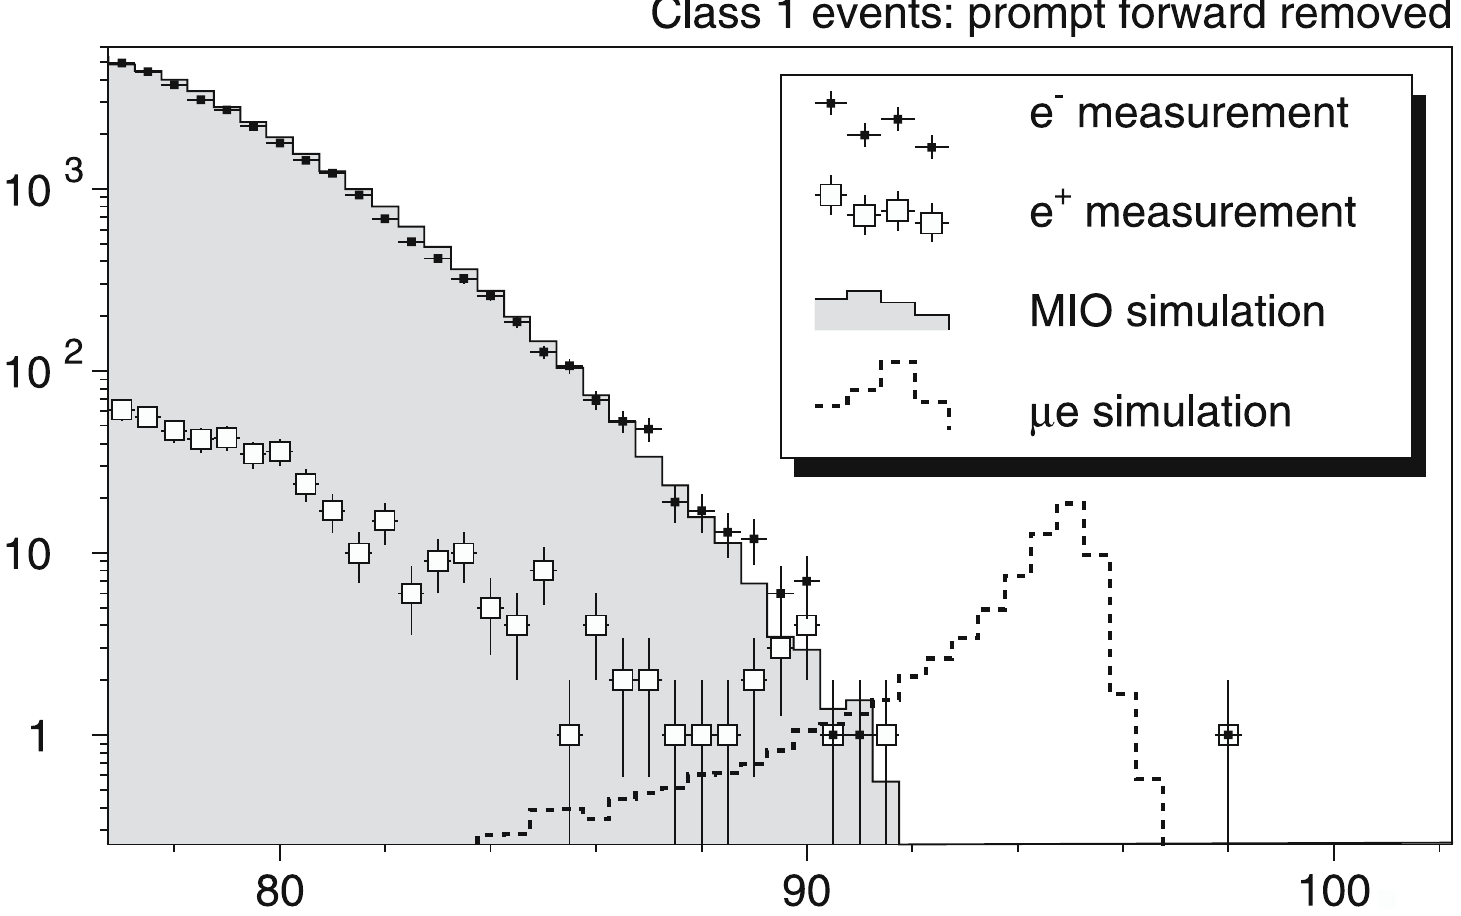
\includegraphics[width=0.8\textwidth, trim = 0 0 0 30,clip]{figures/png/sindrum_ii_2006_fig_11}
    }
  };
  % \node [text width=6cm, scale=0.8] at (4.5,6.4) {mu2e-18894 by Kevin Lynch and Jim Popp};
\end{tikzpicture}
\captionof{figure} {
  \label{fig:sindrum_ii_2006_fig_11}
  SINDRUM-II electron and positron spectra on an \Au{197}\ target from \cite{sindrum_ii:Bertl2006}.
}
\vspace{0.1in}

The positron spectrum shown in Figure \ref{fig:sindrum_ii_2006_fig_11} seems to have
a bump near its high-momentum endpoint. In this note we try to understand what the
implications of this bump are for the Mu2e search for the process of \mumepconv\ .

%%%%%%%%%%%%%%%%%%%%%%%%%%%%%%%%%%%%%%%%%%%%%%%%%%%%%%%%%%%%%%%%%%%%%%%%%%%%%% 
\newpage
\section { Approach}

We start from assuming that the dominant background in the electron channel comes from DIO,
while the positron spectrum is dominated by the positrons from RMC photon conversions.
For \Au{197}, these assumptions hold better for positrons than for electrons:
in the vicinity of 90 MeV, RMC electrons also need to be taken into account.
There are more RMC electrons than positrons (Compton scattering of the RMC photons),
so we just acknowledge the fact, but don't take any action, as the momentum distribution
of the electrons due to Compton scattering is not given in the 2006 paper.

SINDRUM-II used the DIO spectrum on Pb tabulated in \cite{Watanabe_1993} and corrected for the
difference of binding energies in \Au{197} and \Pb{208}.
We use the electron spectrum to develop a simple parameterized model of
the SINDRUM-II detector response. The parameters include the momentum resolution,
assumed to be constant, and the overall reconstruction efficiency dependence on the 
track momentum.

We then use the response model to fit the positron spectrum below 88 MeV/c and
determine the RMC $\kmax$. After that, we can predict the expected background
above 88 MeV/c and quantify the observed excess.

Finally we check if the observed excess is consistent with the signal expected from
\mumepconv\ on \Au{197}.

%%%%%%%%%%%%%%%%%%%%%%%%%%%%%%%%%%%%%%%%%%%%%%%%%%%%%%%%%%%%%%%%%%%%%%%%%%%%%%
%%%%%%%%%%%%%%%%%%%%%%%%%%%%%%%%%%%%%%%%%%%%%%%%%%%%%%%%%%%%%%%%%%%%%%%%%%%%%% 
\newpage
\section {Parameterization of the SINDRUM-II detector response}

%%%%%%%%%%%%%%%%%%%%%%%%%%%%%%%%%%%%%%%%%%%%%%%%%%%%%%%%%%%%%%%%%%%%%%%%%%%%%%
\subsection{Momentum resolution}

Figure ~\ref{fig:dio_1} overlays the electron momentum spectrum measured by SINDRUM-II
and the DIO spectrum on \Pb{208} calculated in \cite{Watanabe_1993} shifted by 0.5 MeV.
It is clear that the two spectra have quite different slopes.
The sign of the difference is easy to understand; in the case of a rapidly falling
spectrum, the finite experimental resolution smears the spectrum and effectively
reduces the observed slope. 

\vspace{0.2in}
\begin{tikzpicture}
  \node[anchor=south west,inner sep=0] at (0,0.) {
    % \node[shift={(0 cm,0.cm)},inner sep=0,rotate={90}] at (0,0) {}
    \makebox[\textwidth][c] {
      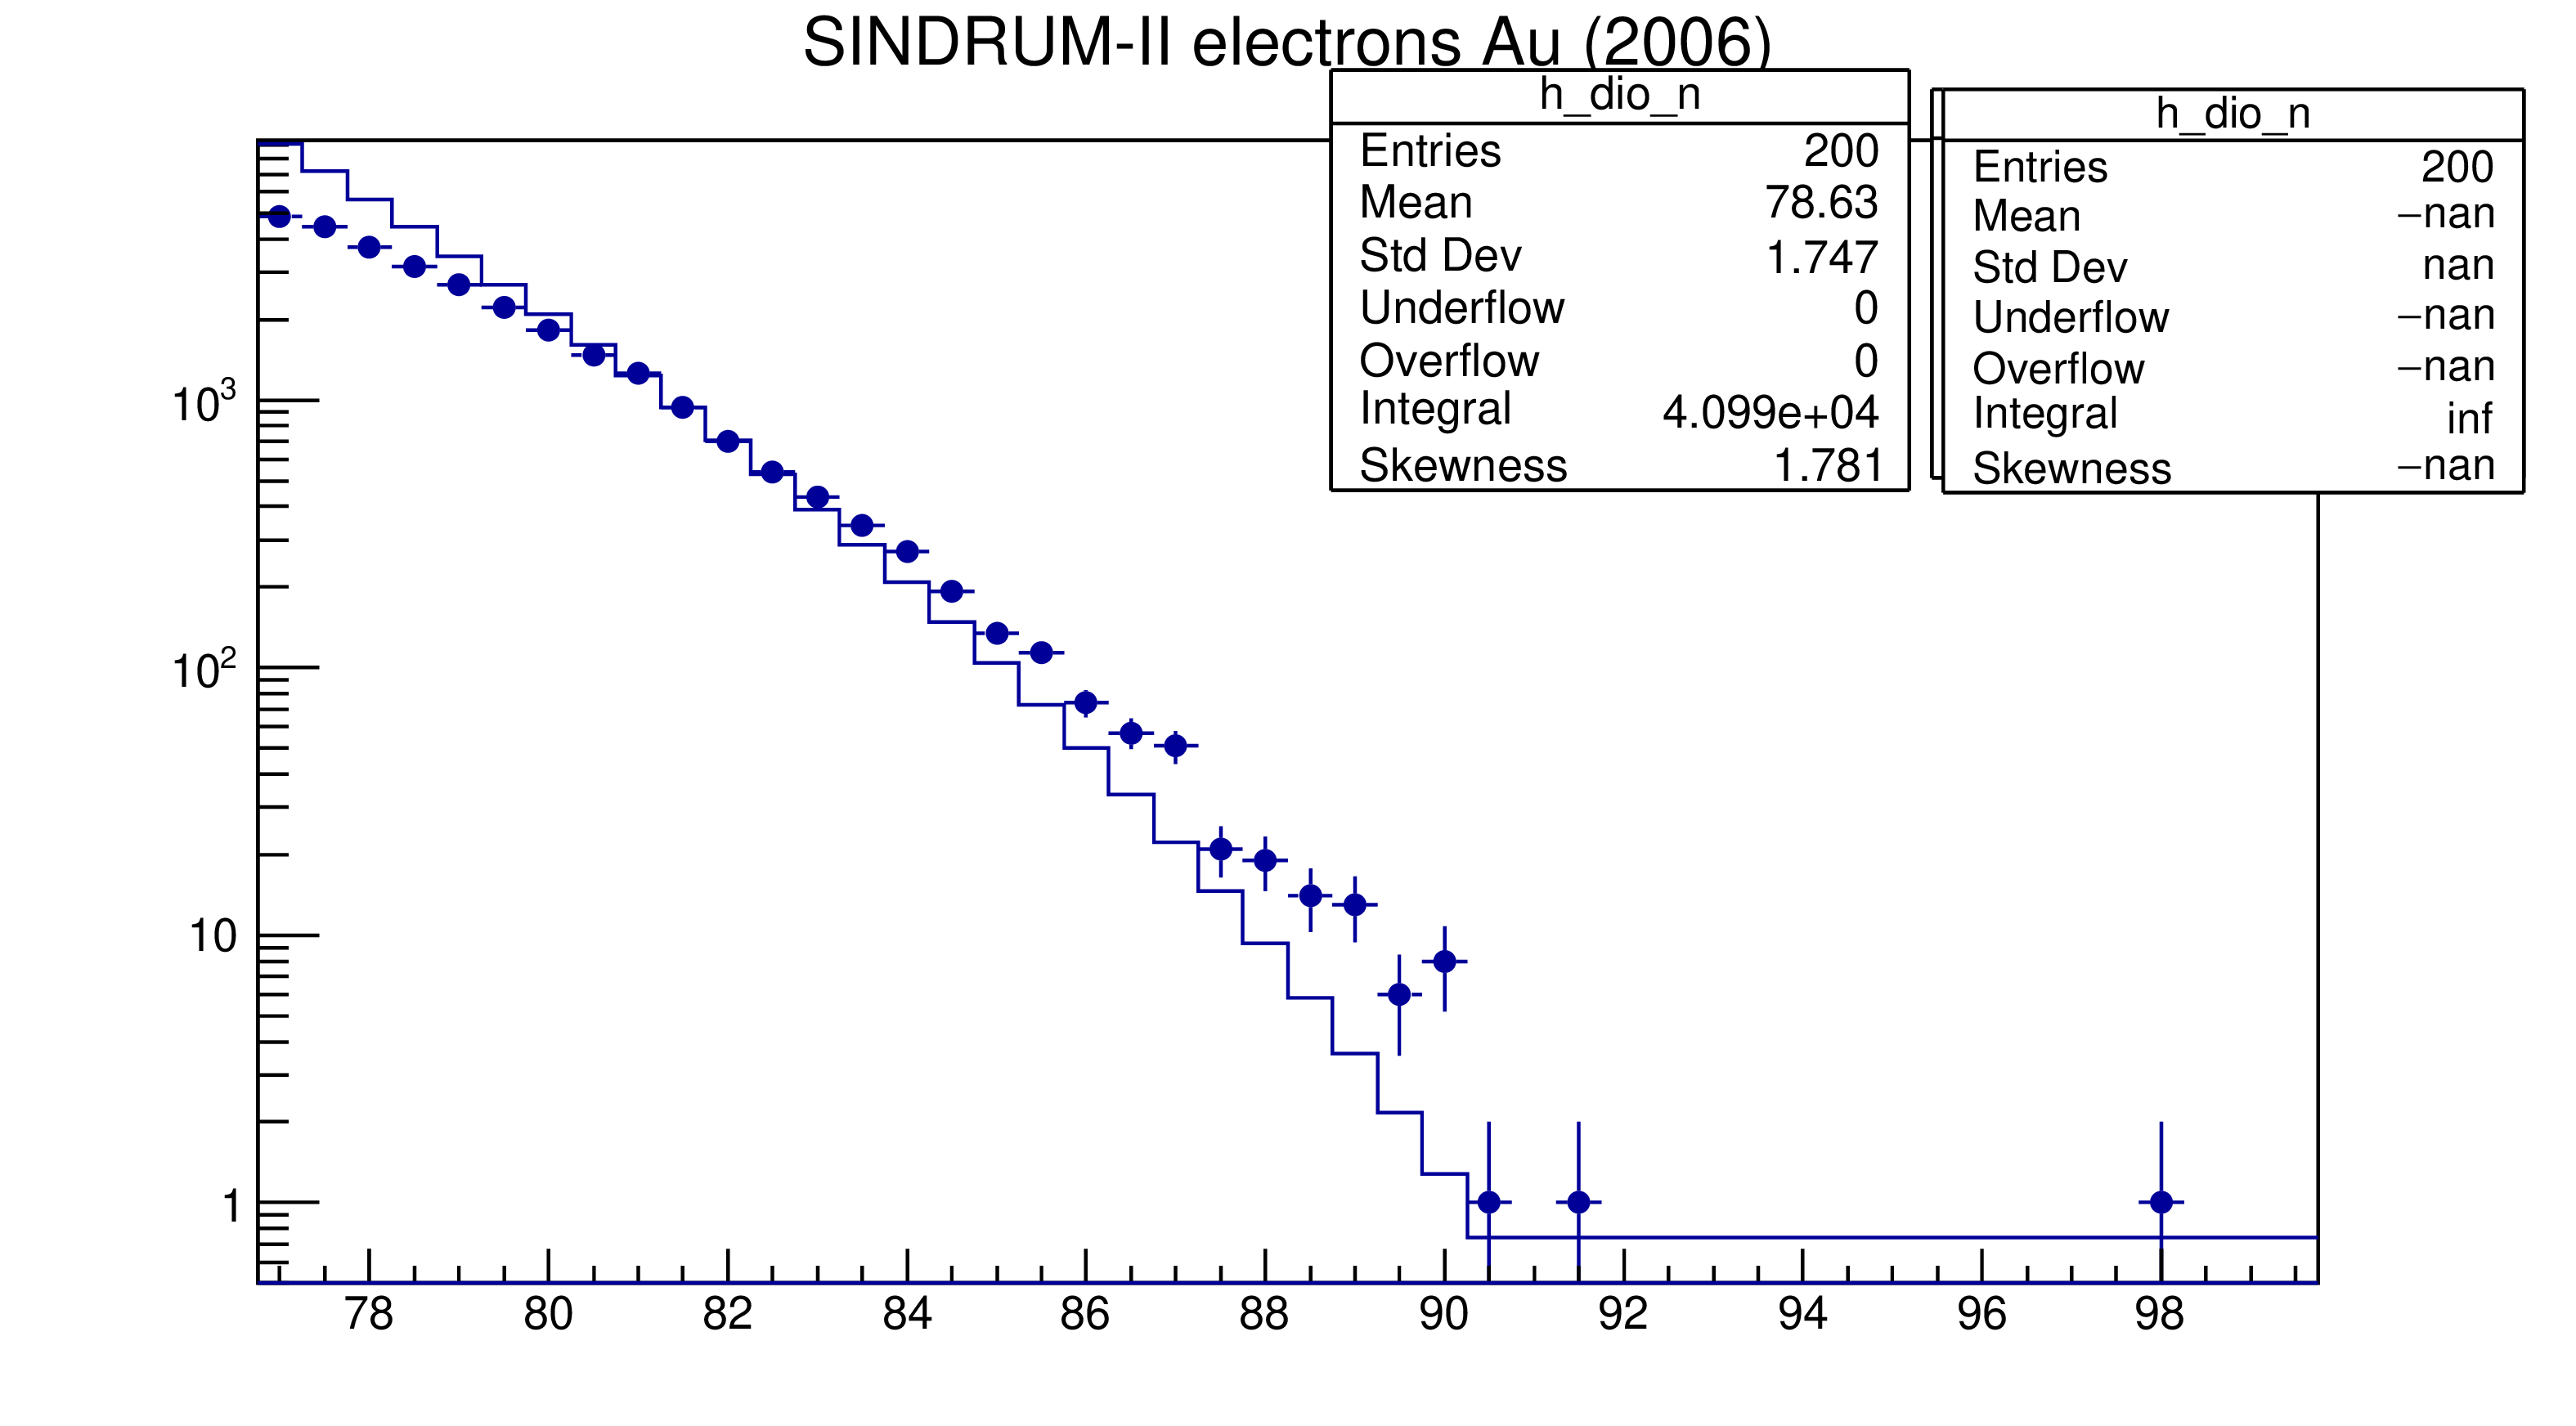
\includegraphics[width=1.0\textwidth]{figures/png/ana_step1_dio_normalized_above_80}
    }
  };
  % \node [text width=6cm, scale=0.8] at (4.5,6.4) {mu2e-18894 by Kevin Lynch and Jim Popp};
\end{tikzpicture}
\captionof{figure} {
  \label{fig:dio_1}
  SINDRUM-II electron spectrum overlaid with the DIO spectrum from \cite{Watanabe_1993}.
  The two spectra are normalized to the same area for p > 80 MeV/c.
}
\vspace{0.2in}

We make a [simplified] assumption that the detector momentum resolution response
is symmetric and can be described by a single Gaussian function. 
The experimental momentum resolution is one of the parameters of the detector response model.
To choose the optimal value, we vary the resolution in the range [1, 3.5] MeV/c, convolve the
theoretical DIO spectrum with the given resolution, and use the resulting distribution to fit
the SINDRUM-II electron spectrum. The fit has one parameter - normalization. The fit $\chi^2$ dependence
on $\sigma_P$ is shown in Figure ~\ref{fig:ana_step1_fit_sigma}, the best value of the resolution
parameter is $\sigma_P = 2.0 \pm 0.1$ MeV/c. This value is significantly higher than the momentum
resolution of the SINDRUM-II detector and is likely due to that contribution of RMC electrons
not accounted for in the procedure. As one can see from Figure ~\ref{fig:sindrum_ii_2006_fig_11},
for momenta close to 90 MeV/c, the contribution of RMC could be non-negligible. As the RMC spectrum
is less steep than the DIO one, ignoring the RMC contribution should result in a larger value of the
best resolution parameter returned by the procedure described above.

\vspace{0.2in}
\begin{tikzpicture}
  \node[anchor=south west,inner sep=0] at (0,0.) {
    % \node[shift={(0 cm,0.cm)},inner sep=0,rotate={90}] at (0,0) {}
    \makebox[\textwidth][c] {
      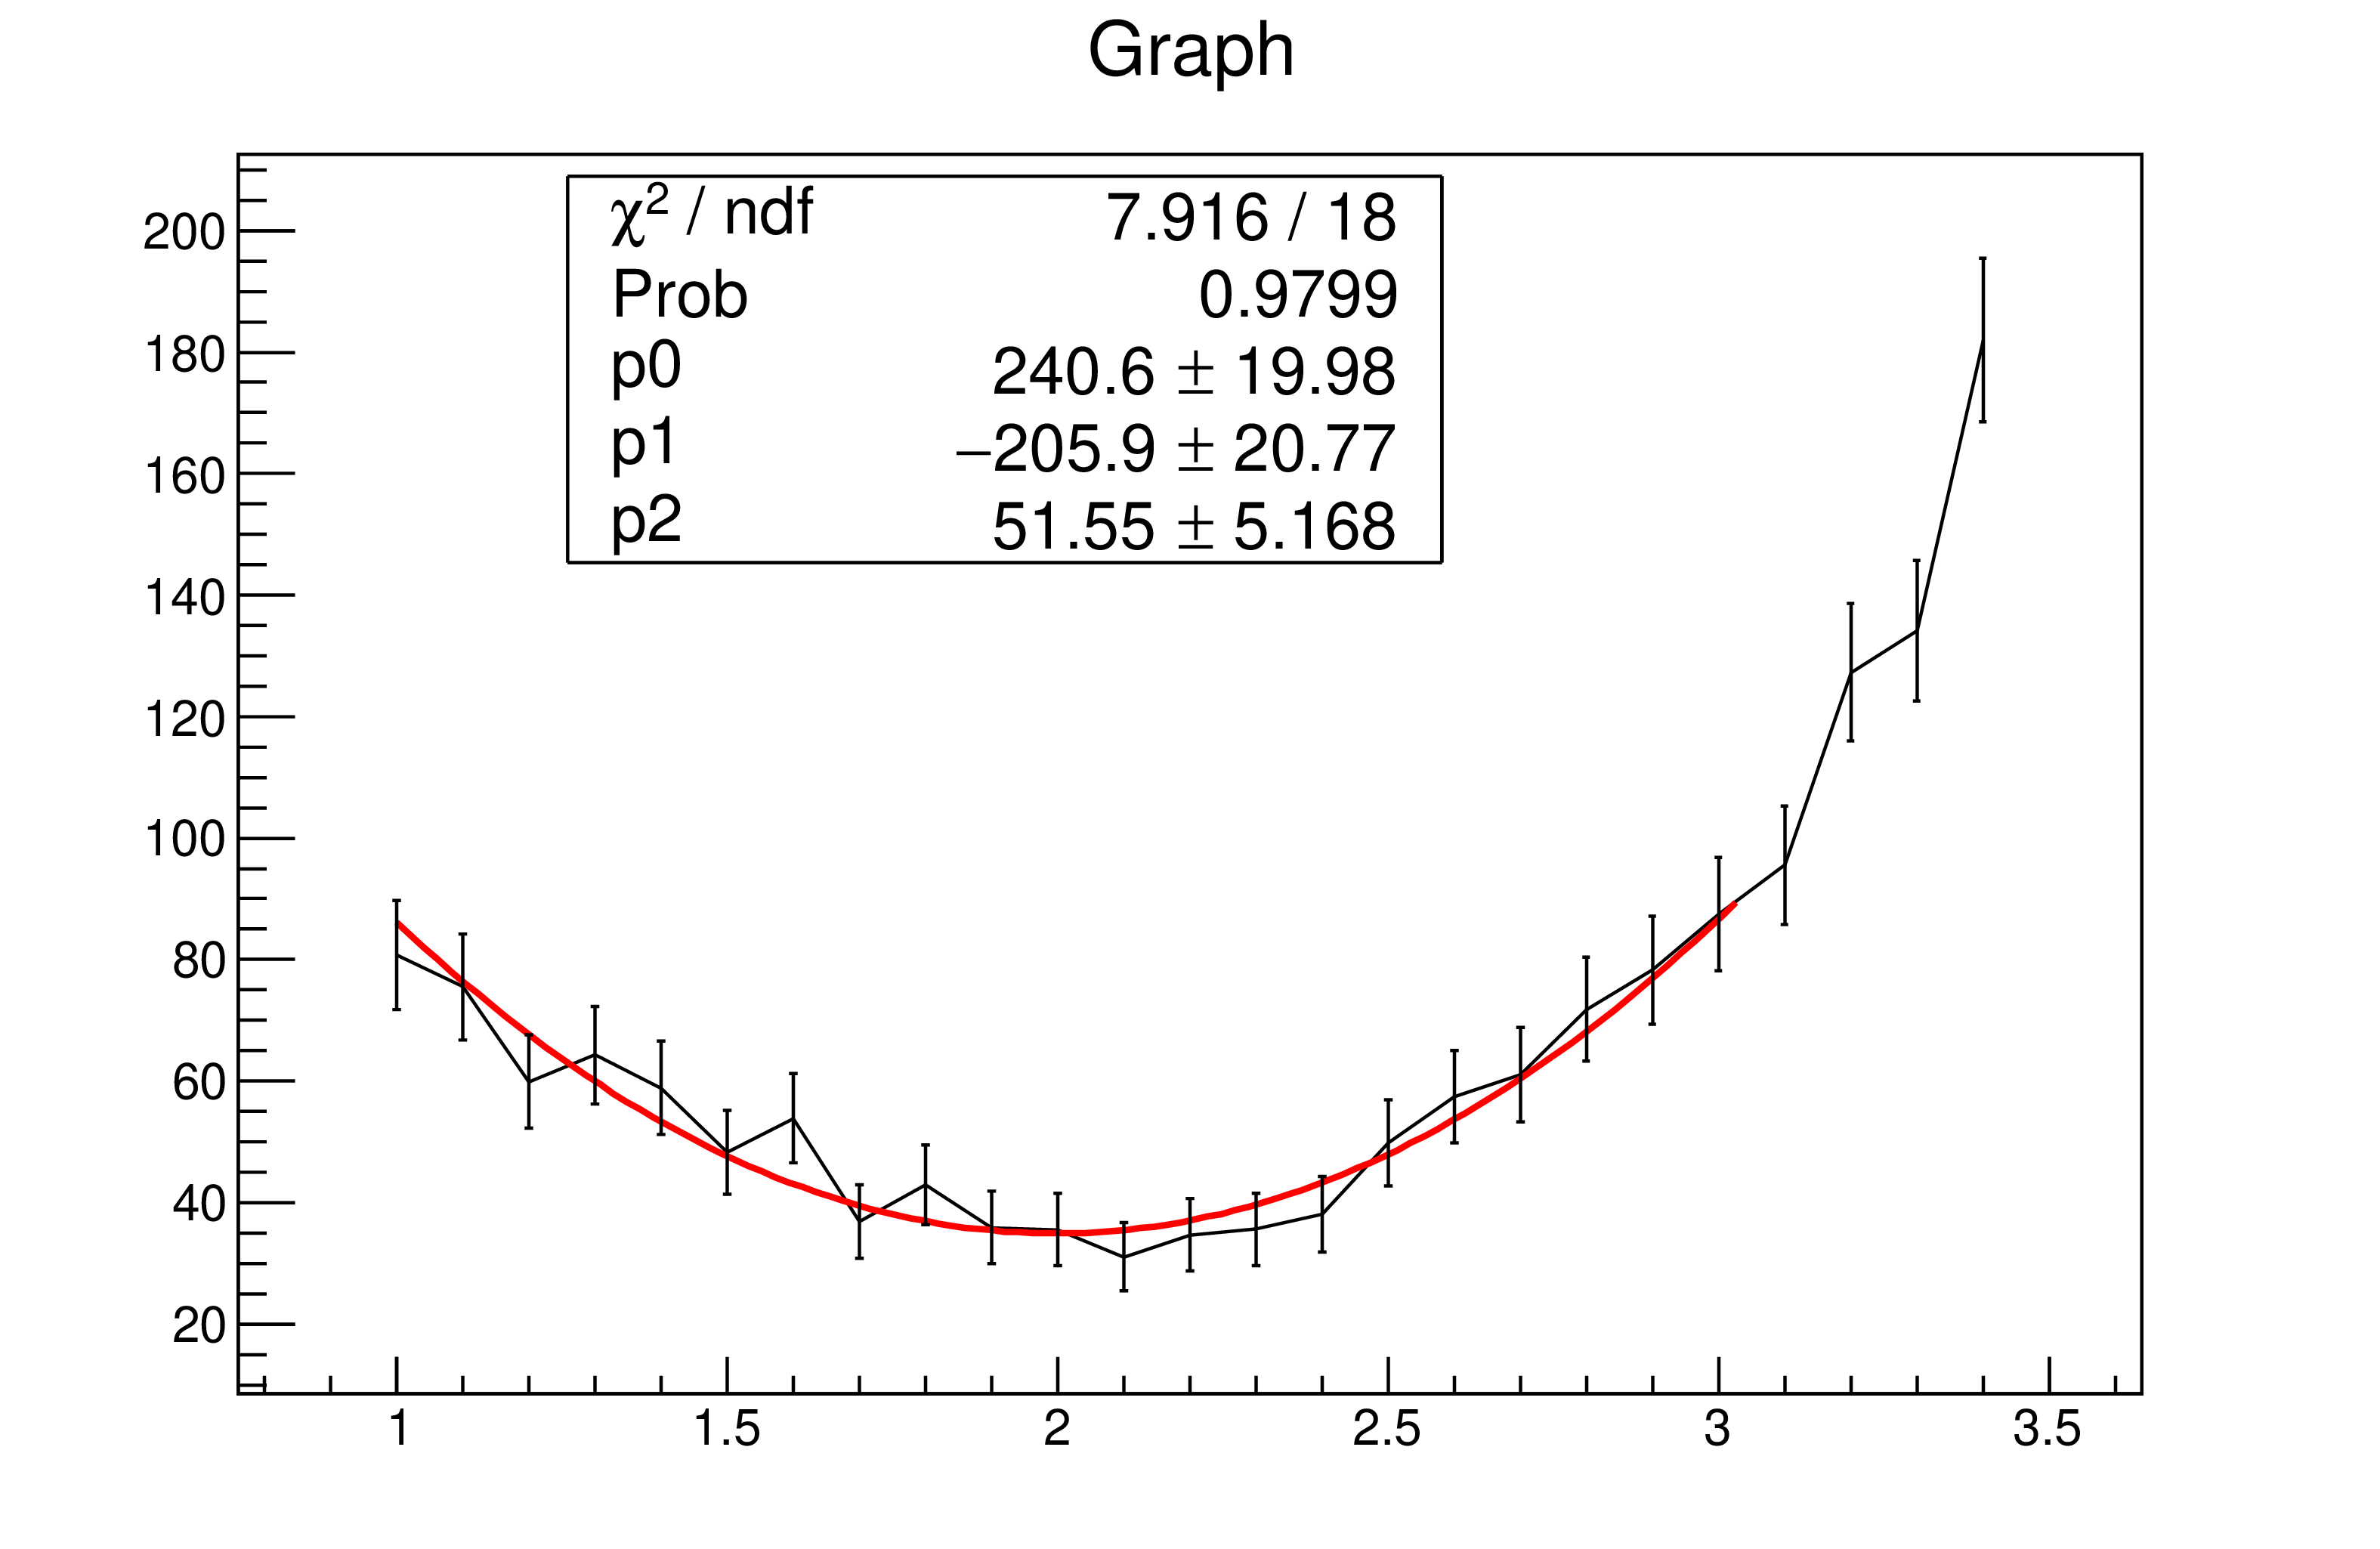
\includegraphics[width=0.9\textwidth, trim = 0 0 0 200, clip]{figures/png/ana_step1_fit_sigma}
    }
  };
  % \node [text width=6cm, scale=0.8] at (4.5,6.4) {mu2e-18894 by Kevin Lynch and Jim Popp};
\end{tikzpicture}
%
\captionof{figure} {
  \label{fig:ana_step1_fit_sigma}
  $\chi^2$ of the fit of the SINDRUM-II DIO electron spectrum with the theoretical distribution
  convolved with a Gaussian with given resolution $\sigma_P$ as a function of $\sigma_P$.
}
\vspace{0.2in}

%%%%%%%%%%%%%%%%%%%%%%%%%%%%%%%%%%%%%%%%%%%%%%%%%%%%%%%%%%%%%%%%%%%%%%%%%%%%%%
\subsection{Tracking efficiency}

To parameterize the SINDRUM-II tracking efficiency, we assume that it is flat
above 80 MeV/c. Normalizing the DIO spectrum convolved with $\sigma_P = 2.0$ MeV/c
resolution to the electron data in the region p > 80 MeV/c and dividing the data spectrum
by the resulting distribution gives the ``efficiency'' dependence on the track momentum
shown in Figure ~\ref{fig:ana_step1_efficiency}. This distribution is fit well by a 
linear efficiency below 80 MeV/c and flat above this.

\begin{tikzpicture}
  \node[anchor=south west,inner sep=0] at (0,0.) {
    % \node[shift={(0 cm,0.cm)},inner sep=0,rotate={90}] at (0,0) {}
    \makebox[\textwidth][c] {
      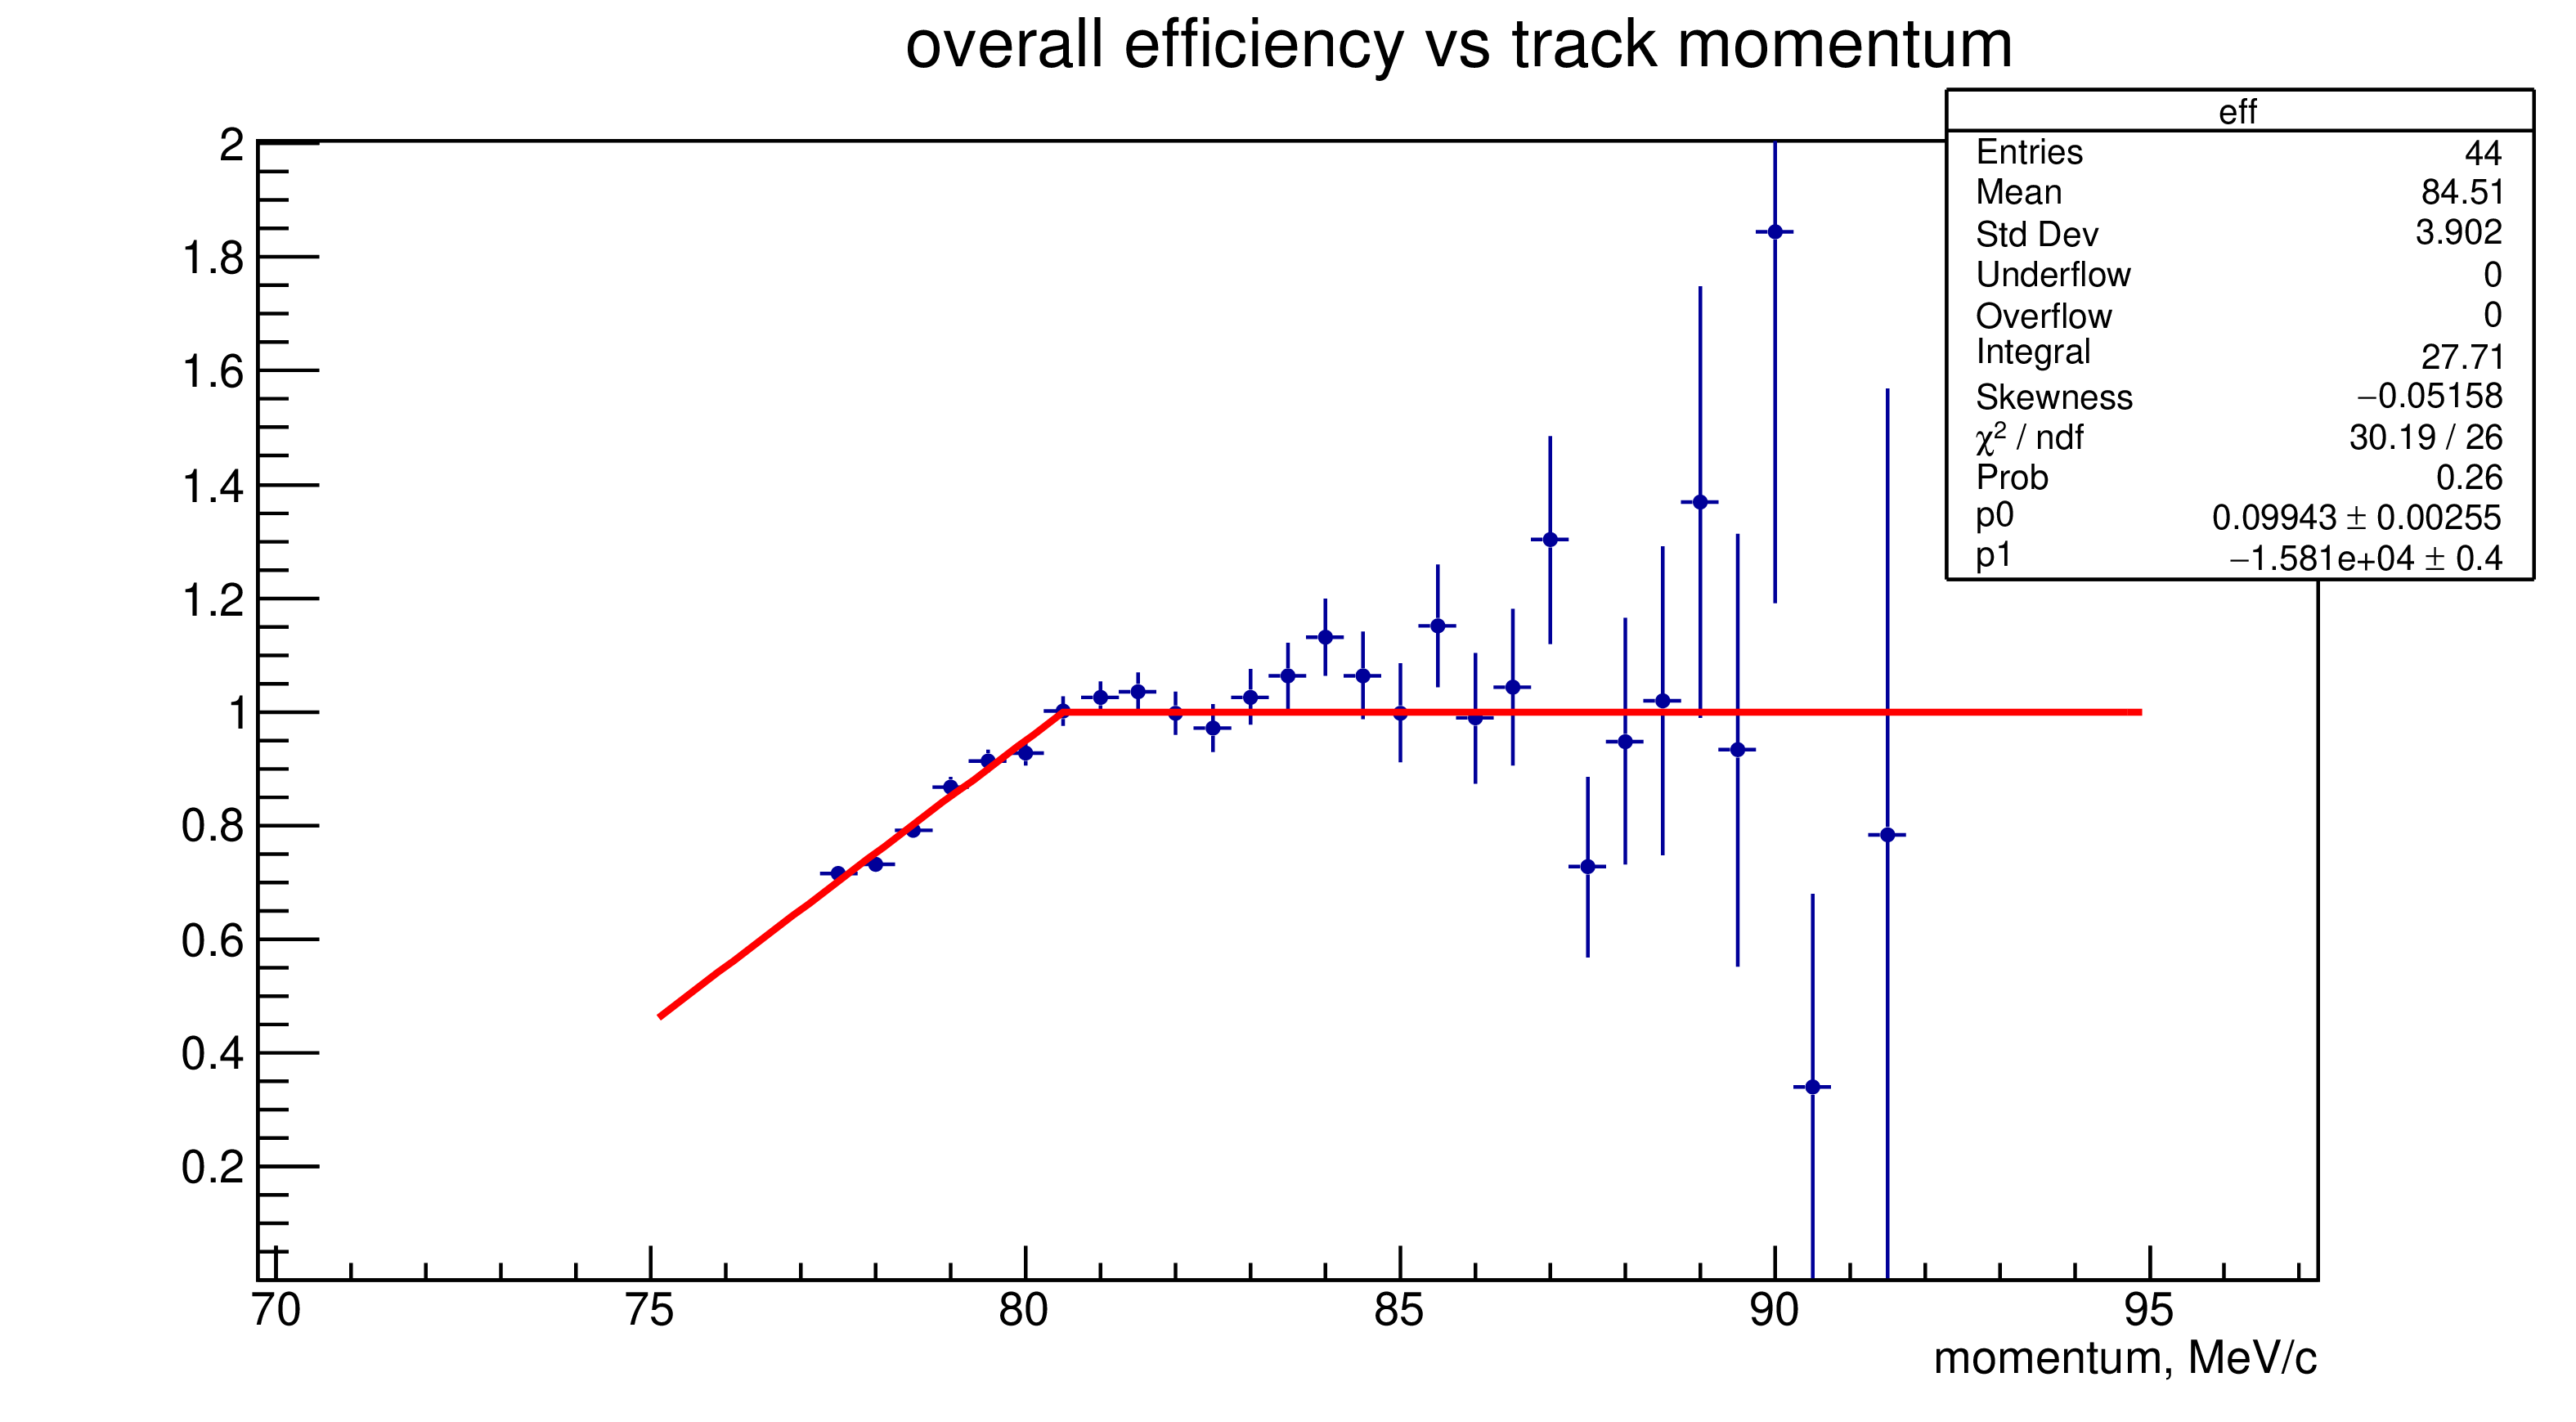
\includegraphics[width=0.9\textwidth]{figures/png/ana_step1_efficiency}
    }
  };
  % \node [text width=6cm, scale=0.8] at (4.5,6.4) {mu2e-18894 by Kevin Lynch and Jim Popp};
\end{tikzpicture}
%
\captionof{figure} {
  \label{fig:ana_step1_efficiency}
  Parameterization of the SINDRUM-II efficiency vs the track momentum.
  Definition of efficiency includes all components - trigger, reconstruction and selection.
  Overall normalization is chosen such that efficiency is equal to one for p > 80 MeV/c.
}
\vspace{0.2in}

This step concludes tuning of the detector response. Figure \ref{fig:ana_step1_best_dio_fit}
shows the description of the electron spectrum with the tuned response.

\vspace{0.2in}
\begin{tikzpicture}
  \node[anchor=south west,inner sep=0] at (0,0.) {
    % \node[shift={(0 cm,0.cm)},inner sep=0,rotate={90}] at (0,0) {}
    \makebox[\textwidth][c] {
      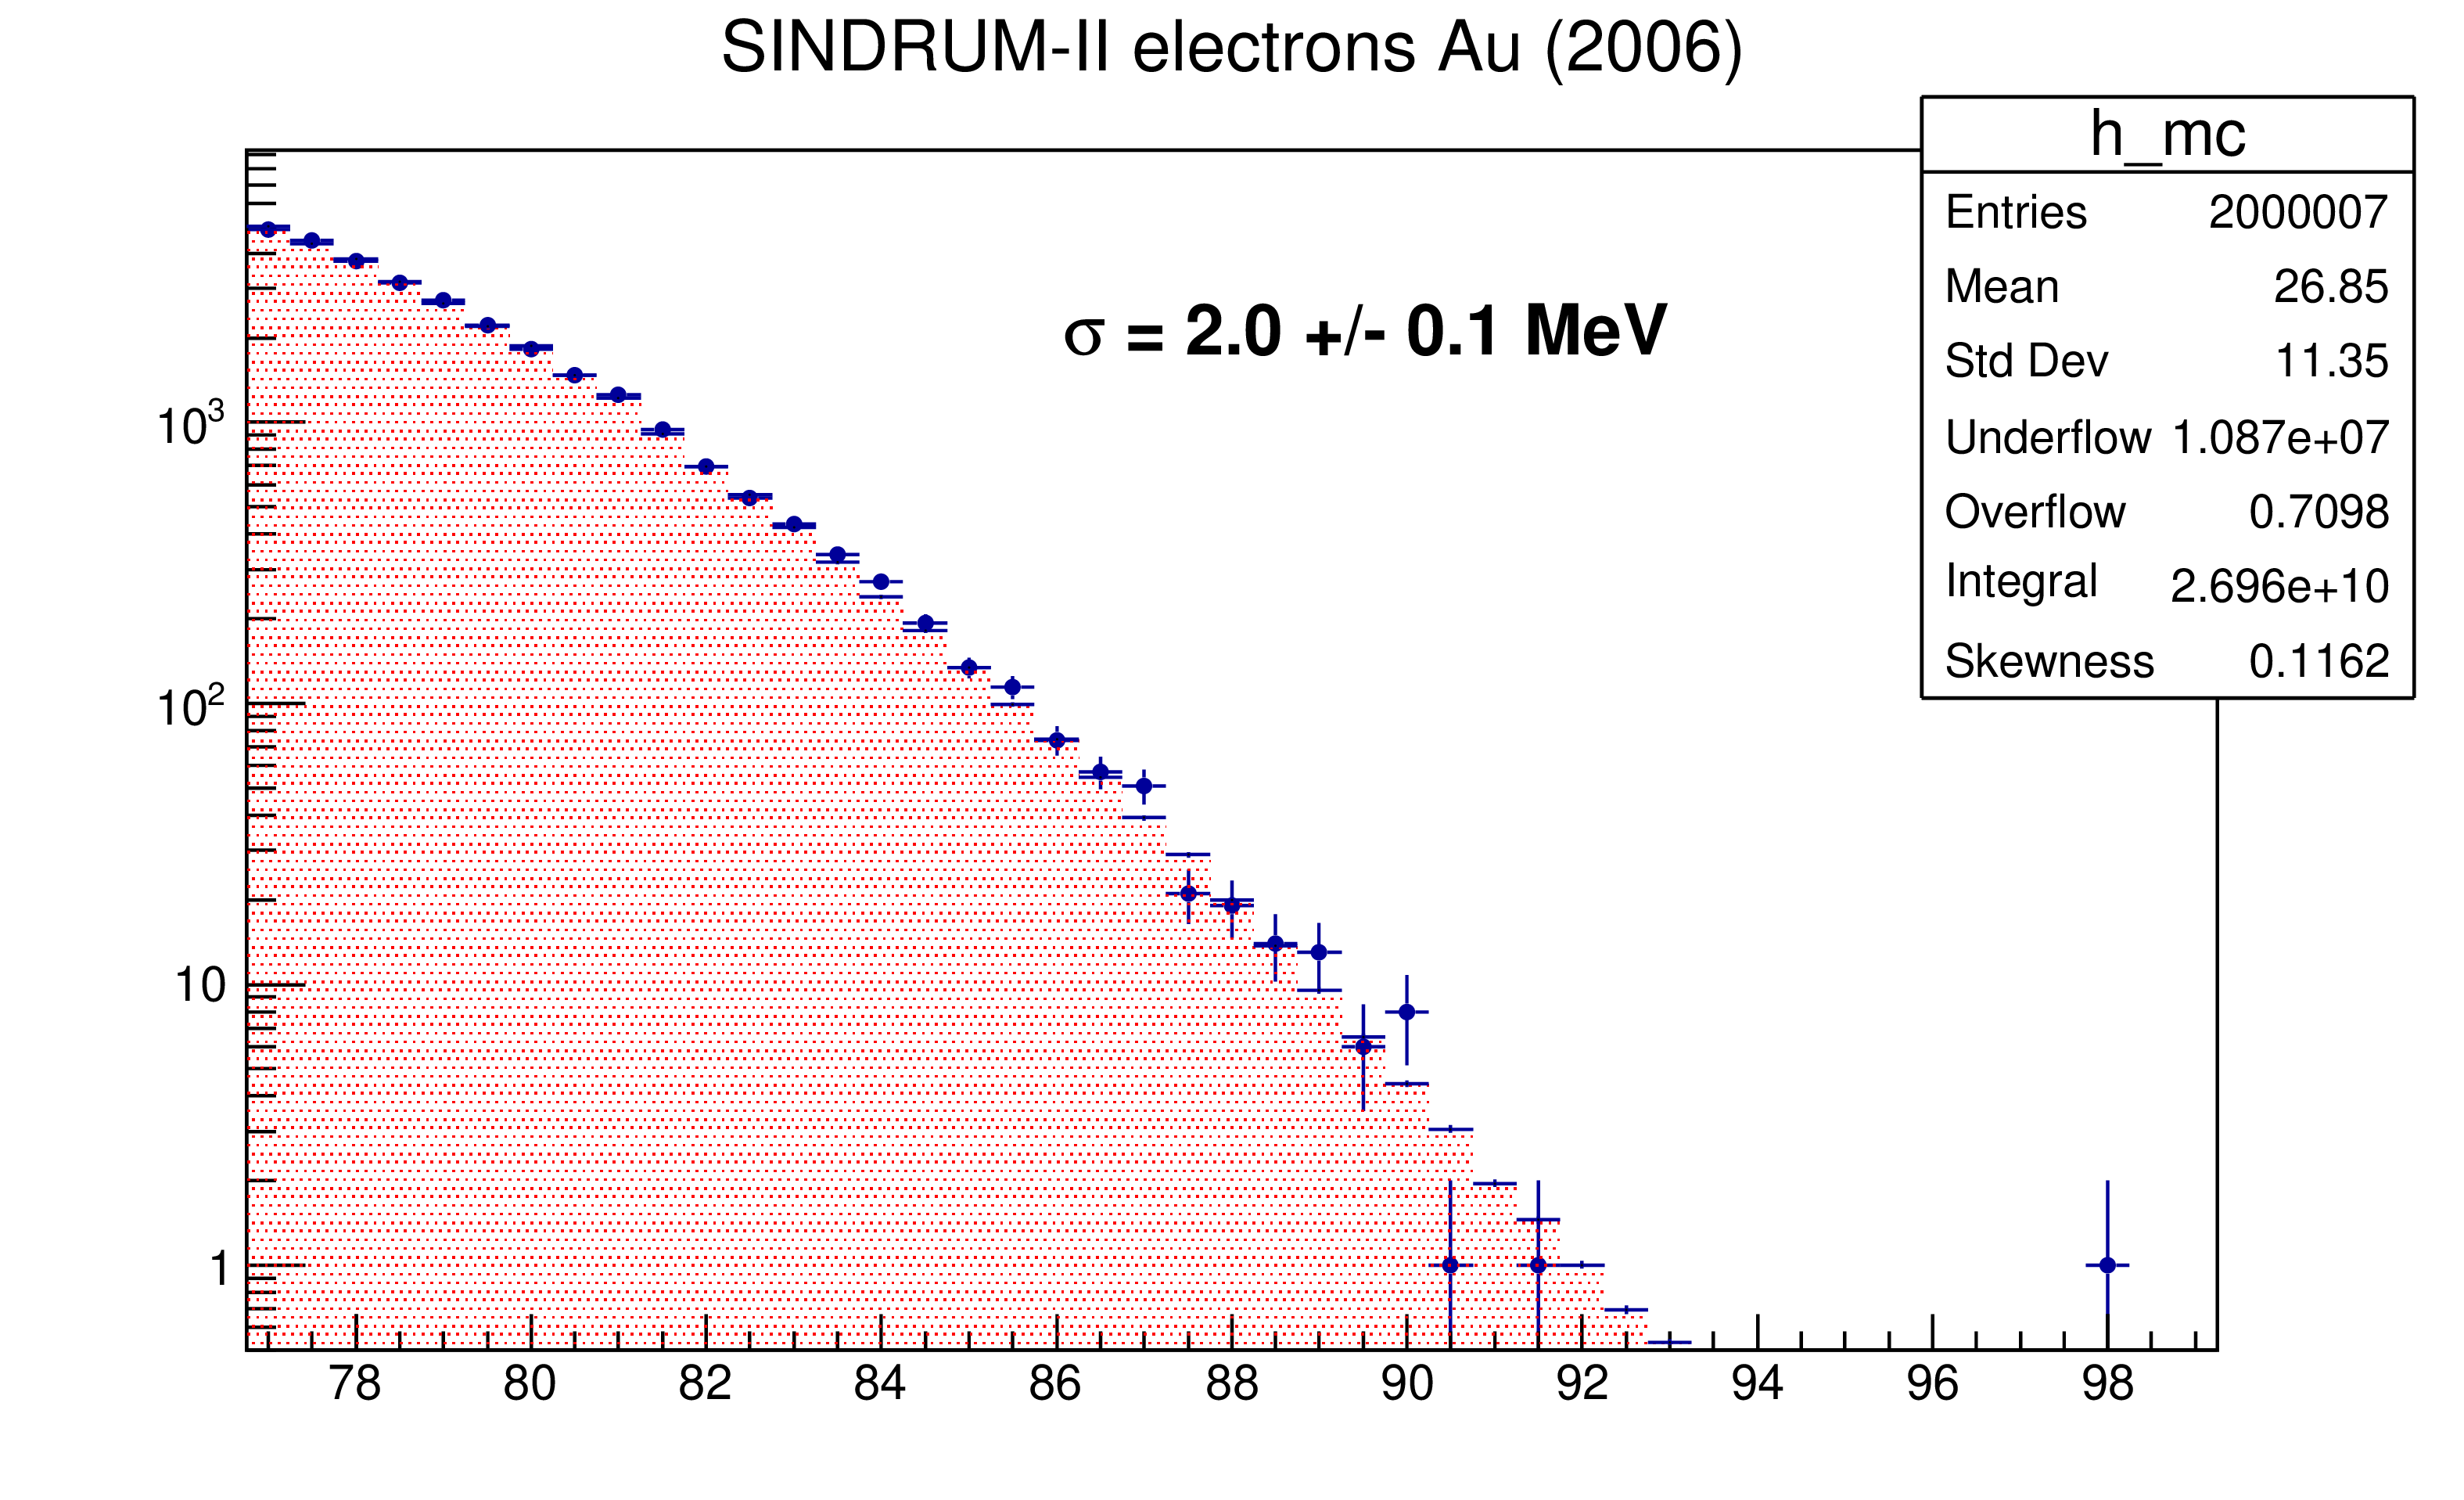
\includegraphics[width=0.99\textwidth]{figures/png/ana_step1_best_dio_fit}
    }
  };
  % \node [text width=6cm, scale=0.8] at (4.5,6.4) {mu2e-18894 by Kevin Lynch and Jim Popp};
\end{tikzpicture}
%
\captionof{figure} {
  \label{fig:ana_step1_best_dio_fit}
  Description of the electron spectrum on the Au target from \cite{sindrum_ii:Bertl2006}
  with the tuned model of the SINDRUM-II detector response.
}

%%%%%%%%%%%%%%%%%%%%%%%%%%%%%%%%%%%%%%%%%%%%%%%%%%%%%%%%%%%%%%%%%%%%%%%%%%%%%% 
\newpage
\section {RMC spectrum and kMax Determination}

Measured RMC photon spectra on nuclei can be successfully described within 
the closure approximation which predicts the RMC photon spectrum depending
on just one parameter - the photon spectrum endpoint:
$$
    \frac{dN}{dE} ~=~ \frac{e^2}{\pi} \frac{k_m^2}{ m_{\mu}^2} (1 - \alpha) (1-x+2x^2)x(1-x)^2
$$
, where E is the photon energy, $k_m$ is the energy spectrum endpoint, $\rm \alpha = (N-Z)/A$,
and $x = E/k_m$ \cite{Christillin_1980}.

Values of $k_m$ for different nuclei are not predicted, but determined from the fits
to experimental data. Typically, fits return $k_m$ values significantly lower that
the kinematically allowed limits. 

We determine the $\bf k_m$ by fitting the SINDRUM-II positron spectrum with a closure approximation spectrum convoluted with the resolution $\sigma_P = 2$ MeV and the
efficiency determined from the fit to the electron spectrum and varying the value
of $\bf k_m$. Results of the fit are shown in Figure ~\ref{fig:ana_step2_fit_kmax},
the best fit is provided by $\bf k_m = 88.0 \pm 0.6$ MeV.

With the energy losses taking into account, the value becomes  $k_m = 88.6 \pm 0.6$ MeV.
Maximal photon energy allowed in  $\mu \Au{197}$(GS) $\rm \rightarrow \nu \gamma ^{197}Pt$(GS)
transition is 93.8 MeV.

\vspace{0.1in}
\begin{tikzpicture}
  \node[anchor=south west,inner sep=0] at (0,0.) {
    % \node[shift={(0 cm,0.cm)},inner sep=0,rotate={90}] at (0,0) {}
    \makebox[\textwidth][c] {
      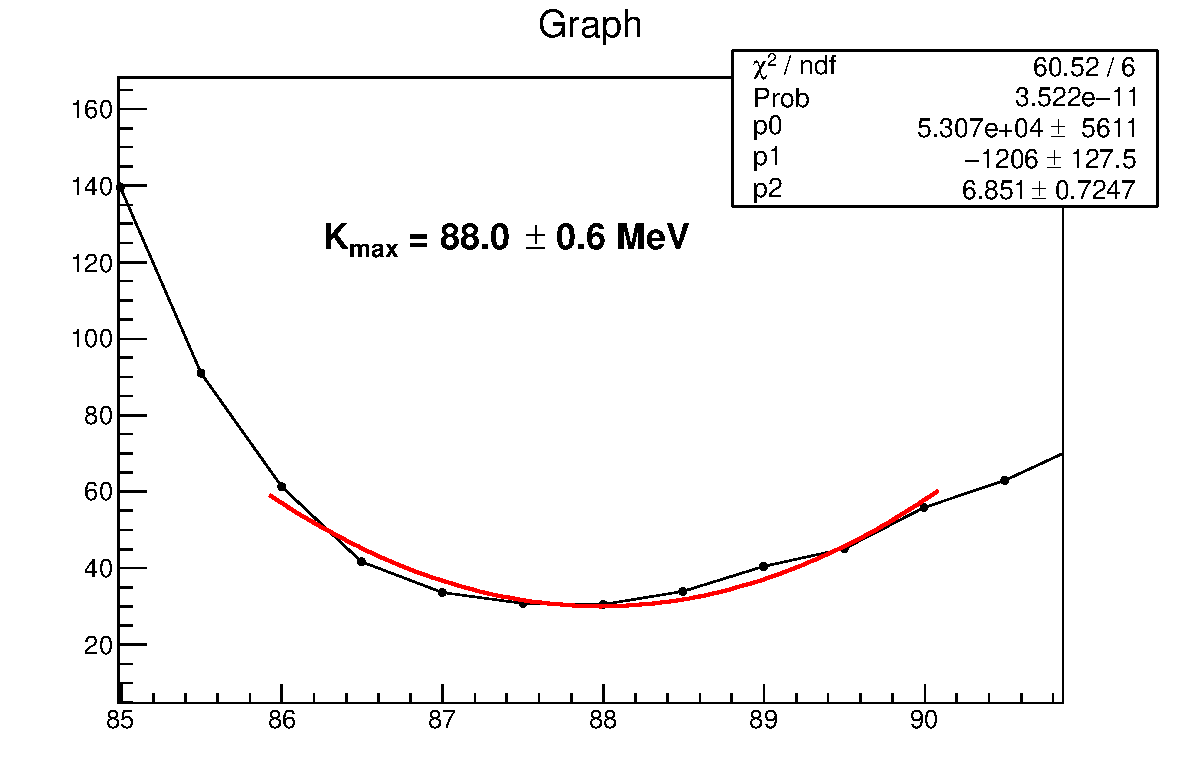
\includegraphics[width=1.0\textwidth]{figures/pdf/ana_step2_fit_kmax}
    }
  };
  % \node [text width=6cm, scale=0.8] at (4.5,6.4) {mu2e-18894 by Kevin Lynch and Jim Popp};
\end{tikzpicture}
\captionof{figure} {
  \label{fig:ana_step2_fit_kmax}
  $\bf k_m$ fit of the SINDRUM-II positron spectrum, energy losses are not
  taken into account
}
\vspace{0.1in}


Figure \ref{fig:ana_step2_ppos_best_fit} overlays the SINDRUM-II positron spectrum on
\Au{197}\ target with the closure approximation spectrum convoluted with the 
parameterized model of the SINDRUM-II detector response.

There are 14 events above 88 MeV in the data.

Looking at the data above 94 MeV, we can estimate the background due to radiative
pion capture (RPC) and cosmics to be of the order of one event.
Prediction of the closure approximation-based RMC model gives significantly less
than one event.

We therefore need to ask whether the closure approximation gives a reliable
description of the RMC positron spectrum near the end point. The closure approximation
doesn't take into account transitions to the exclusive low-lying states of the daughter
nucleus.

In case of the \Au{197} target, a transition \Au{197} --> $^{197}Pt$ to
the ground state of Pt nucleus is allowed. Given that the energy splitting between
an electron and a positron from the photon conversion is almost uniform,
the positron spectrum corresponding to such a transition, in a first approximation,
should be flat. 

probability of the order of $10^-3$, 

\vspace{0.1in}
\begin{tikzpicture}
  \node[anchor=south west,inner sep=0] at (0,0.) {
    % \node[shift={(0 cm,0.cm)},inner sep=0,rotate={90}] at (0,0) {}
    \makebox[\textwidth][c] {
      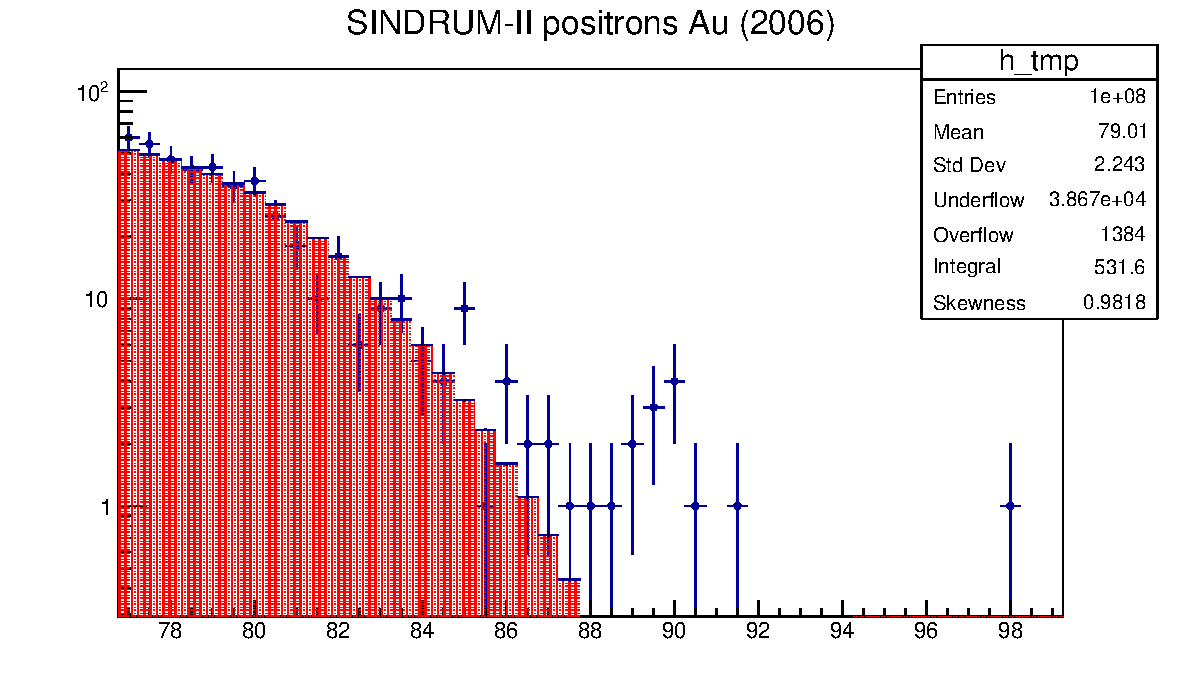
\includegraphics[width=1.0\textwidth]{figures/pdf/ana_step2_ppos_best_fit}
    }
  };
  % \node [text width=6cm, scale=0.8] at (4.5,6.4) {mu2e-18894 by Kevin Lynch and Jim Popp};
\end{tikzpicture}
\captionof{figure} {
  \label{fig:ana_step2_ppos_best_fit}
  best fit of the SINDRUM-II positron spectrum with closure approximation spectrum 
  convoluted with the parameterized model of the SINDRUM-II detector response
}
\vspace{0.1in}

%%%%%%%%%%%%%%%%%%%%%%%%%%%%%%%%%%%%%%%%%%%%%%%%%%%%%%%%%%%%%%%%%%%%%%%%%%%%%%
\subsection{Final states with the broken down  daughter nucleus}

As the daughter nucleus can break down, one could ask whether photons from
transitions
$$
\mu + \Au{197} \rightarrow \gamma + \nu + ^{197-k}Pt + k \rm neutrons
$$
or 
$$
\mu + \Au{197} \rightarrow \gamma + \nu + ^{197-k}A_{Z=79-k} + k \rm protons
$$

could have a higher spectrum end point. Figure ~\ref{fig:pt197_dmass} shows the
mass differences for the two different schenarios, 
  
\vspace{0.1in}
\begin{tikzpicture}
  \node[anchor=south west,inner sep=0] at (-2.0,0.0) {
    % \node[shift={(0 cm,0.cm)},inner sep=0,rotate={90}] at (0,0) {}
    % \makebox[\textwidth][c] {
      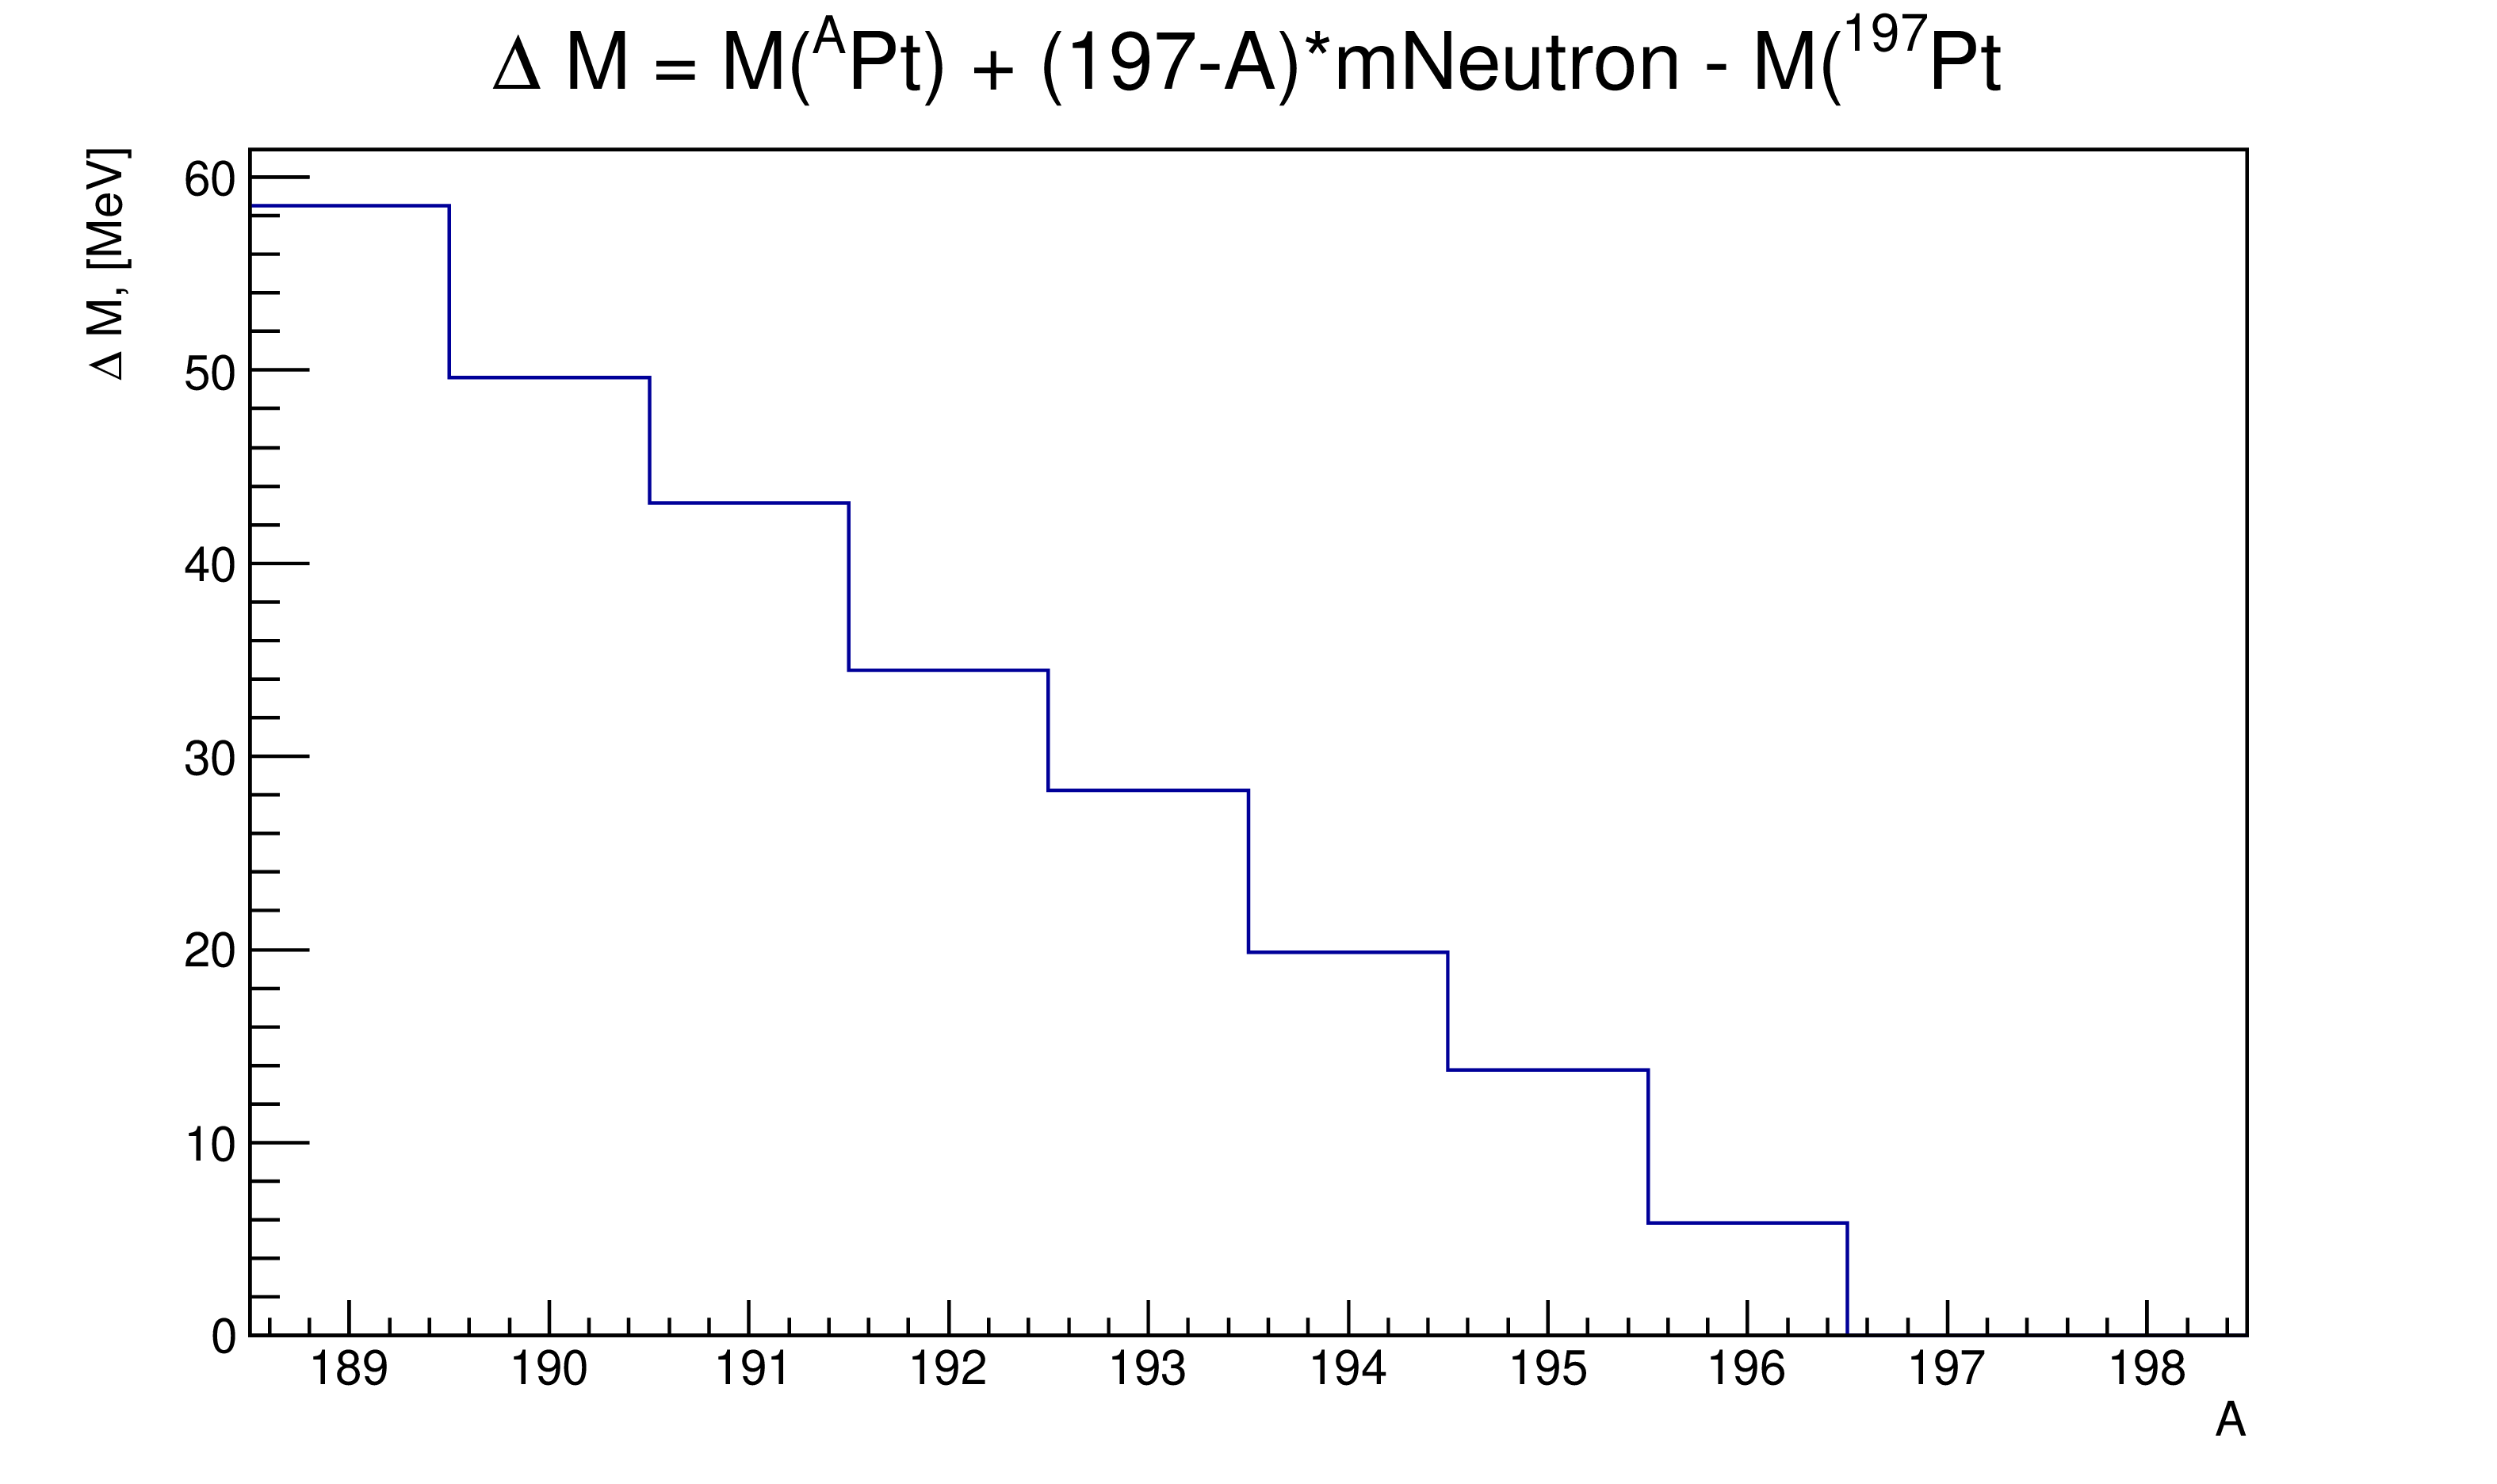
\includegraphics[width=0.6\textwidth]{figures/png/pt197_dmass}
    % }
  };
  \node[anchor=south west,inner sep=0] at (6.0,0.0) {
    % \node[shift={(0 cm,0.cm)},inner sep=0,rotate={90}] at (0,0) {}
    % \makebox[\textwidth][c] {
      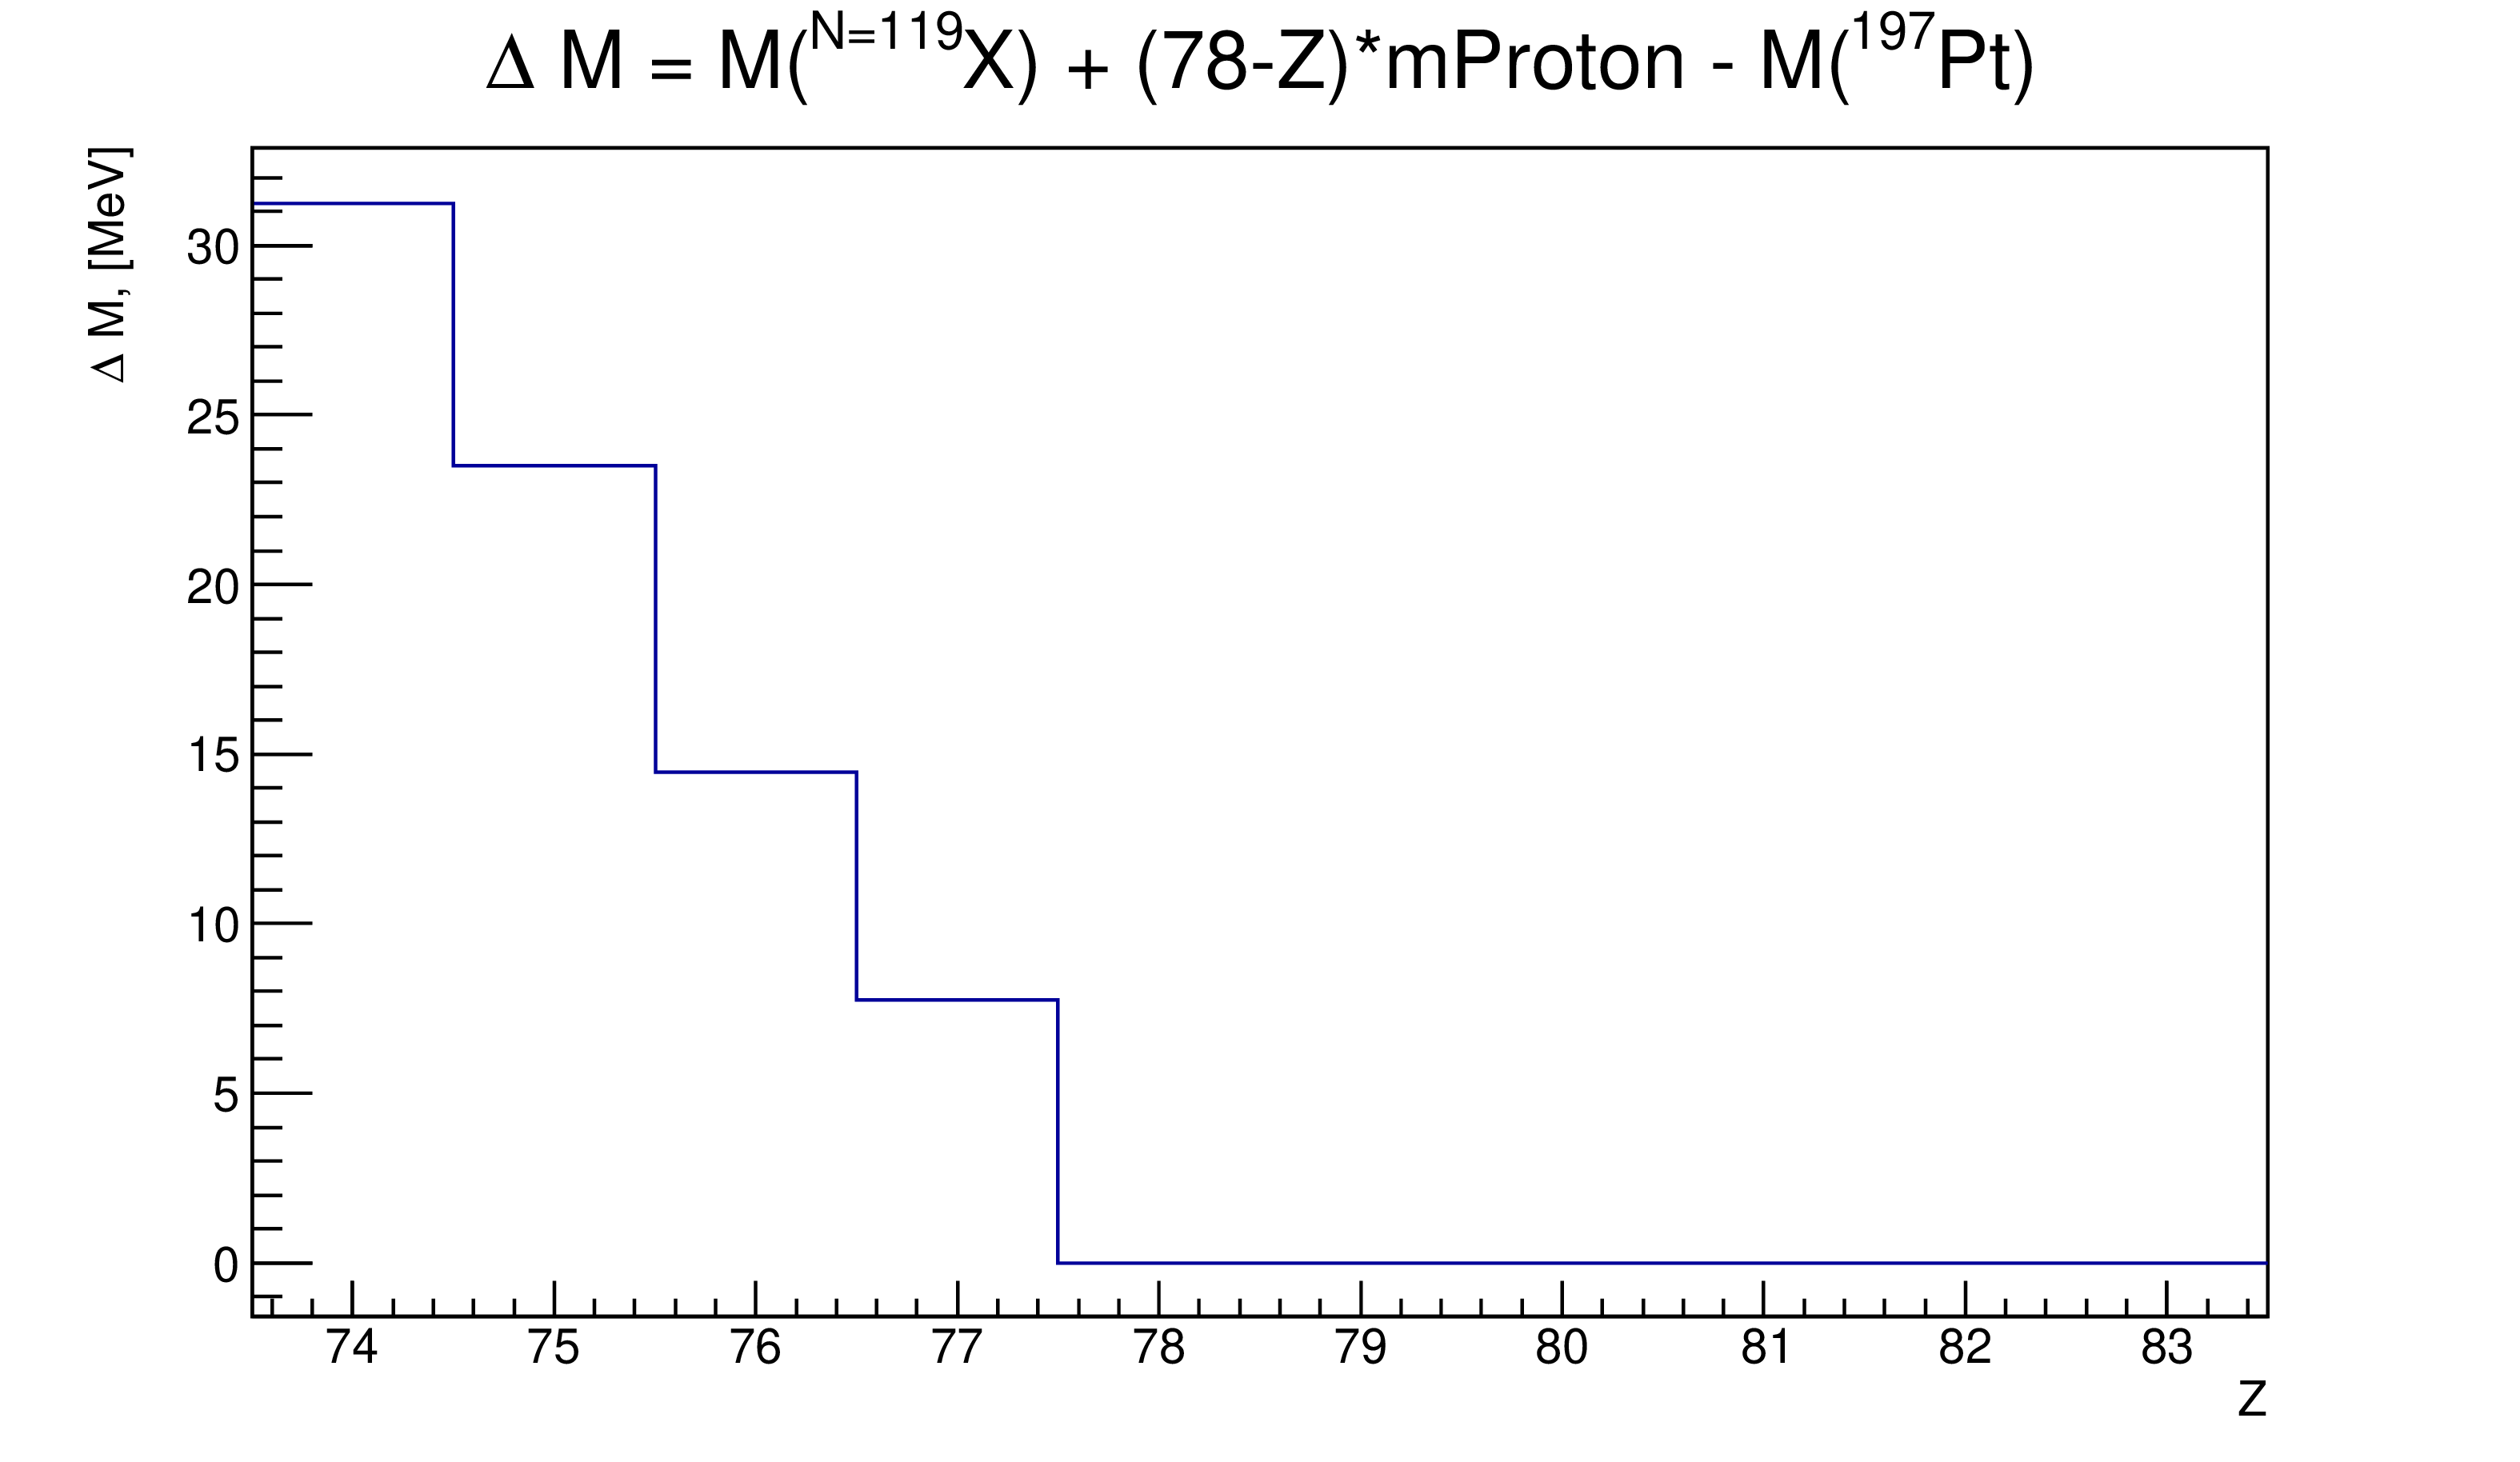
\includegraphics[width=0.6\textwidth]{figures/png/pt197_dmass_n}
    % }
  };
  % \node [text width=6cm, scale=0.8] at (4.5,6.4) {mu2e-18894 by Kevin Lynch and Jim Popp};
\end{tikzpicture}
\captionof{figure} {
  \label{fig:pt197_dmass}
  Mass differences between the final state with the broken down daughter nucleus
  and $^{197} Pt$ for different breakdown scenarios.
  The final state with ``unbroken'' $^{197} Pt$ always has the lowest mass and,
  therefore, the highest photon spectrum endpoint
}
\vspace{0.1in}

%%% Local Variables:
%%% mode: latex
%%% TeX-master: t
%%% End:

%%%%%%%%%%%%%%%%%%%%%%%%%%%%%%%%%%%%%%%%%%%%%%%%%%%%%%%%%%%%%%%%%%%%%%%%%%%%%% 
\newpage
\section {SINDRUM-II momentum scale }

In \cite{sindrum_ii:Bertl2006}, the momentum scale has been calibrated using
the edge of the Michel spectrum from muon decays $\mu^+ \rightarrow e^+ \nu \bar{\nu}$
at rest. The calibration has been performed with the magnetic field reduced to about 50\%
of the nominal value. The reconstructed positron momentum distribution is shown
in Figure \ref{fig:sindrum_ii_fig_08_fit}.

{\bf replace electrons with positrons in the title below}

\vspace{0.1in}
\begin{tikzpicture}
  \node[anchor=south west,inner sep=0] at (0,0.) {
    % \node[shift={(0 cm,0.cm)},inner sep=0,rotate={90}] at (0,0) {}
    \makebox[\textwidth][c] {
      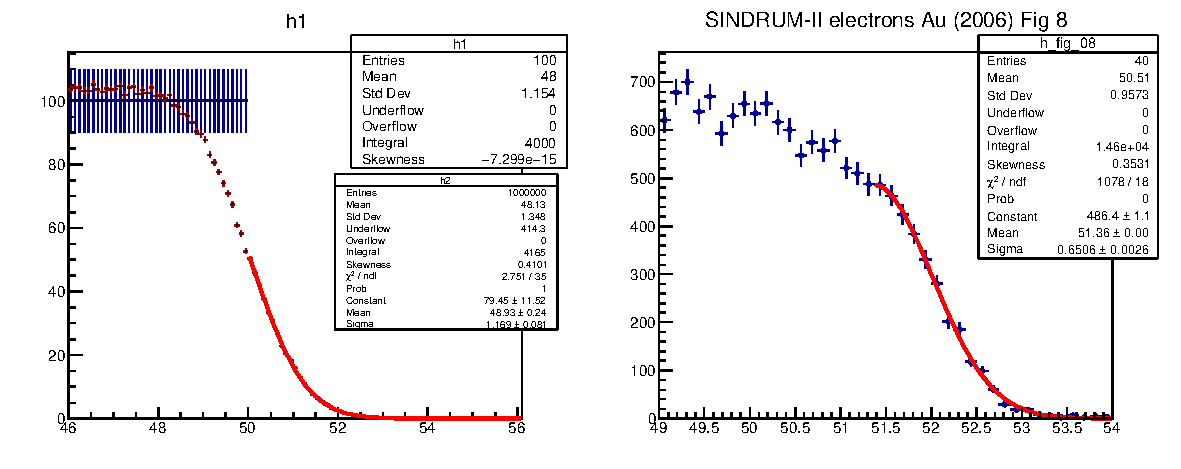
\includegraphics[width=0.99\textwidth]{figures/pdf/sindrum_ii_fig_08_fit}
    }
  };
  % \node [text width=6cm, scale=0.8] at (4.5,6.4) {mu2e-18894 by Kevin Lynch and Jim Popp};
\end{tikzpicture}
\captionof{figure} {
  \label{fig:sindrum_ii_fig_08_fit}
  Reconstructed momentum spectrum of positrons from $\mu^+ \rightarrow e^+ \nu \bar{\nu}$
  decays used in \cite{sindrum_ii:Bertl2006} for detector momentum calibration.
}
\vspace{0.1in}

Although radiative corrections modify the positron spectrum, as shown in Figure \ref{fig:mu2e_5645_fig_001_mue3_decay} their impact on the edge of the Michel spectrum
is fairly small, and the reconstructed position and shape of the edge depend primarily
on the energy losses and the momentum resolution.

\begin{tikzpicture}
  \node[anchor=south west,inner sep=0] at (0,0.) {
    % \node[shift={(0 cm,0.cm)},inner sep=0,rotate={90}] at (0,0) {}
    \makebox[\textwidth][c] {
      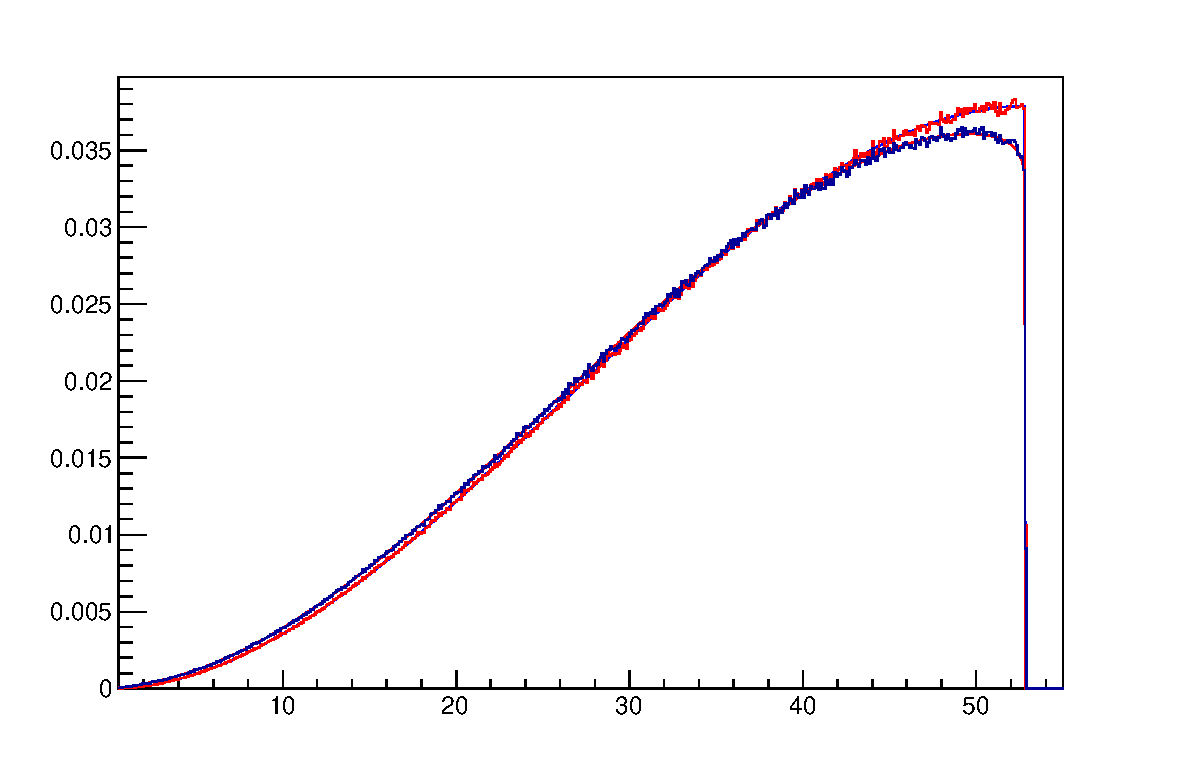
\includegraphics[width=0.99\textwidth]{figures/pdf/mu2e_5645_fig_001_mue3_decay}
    }
  };
  % \node [text width=6cm, scale=0.8] at (4.5,6.4) {mu2e-18894 by Kevin Lynch and Jim Popp};
\end{tikzpicture}
\captionof{figure} {
  \label{fig:mu2e_5645_fig_001_mue3_decay}
  Monte Carlo momentum spectrum of positrons from the $\mu^+ \rightarrow e^+ \nu \bar{\nu}$
  decay. Red: leading order, Blue: with radiative corrections taken into account.
}
\vspace{0.1in}

We expect the positron momentum referred to in the paper
to be the momentum in the first reconstructed point on the trajectory. As such, the
reconstructed Michel edge should be affected by the energy losses in front of the
tracker, their fluctuations, as well as the momentum resolution of the tracker.
According to \cite{sindrum_ii:Bertl2006}, the energy losses in front of the tracker are due to 
losses in the Au target (75 mg/cm$^2$) and the wall of the vacuum chamber (324 mg/cm$^2$),
main components of which are aluminum and carbon fiber.

To validate our understanding of the SINDRUM-II momentum calibration,
we simulate energy losses of positrons with initial momenta distributed uniformly
in the range [45,52.8] MeV/c in a structure consisting of the two layers described
above. The initial momentum distribution is shown
in Figure ~\ref{fig:sindrum_ii_michel_calibration} in red,
the positron momentum distribution on exit from the vacuum chamber wall is shown in blue.

{\bf Currently not shaded, need another iteration on the figure}

Shaded is the positron momentum distribution on exit convolved with
a Gaussian with $\sigma = 0.55$ MeV/c corresponding to the SINDRUM-II
momentum resolution of 1.3 MeV/c FWHM \cite{sindrum_ii:Kaulard1997_Thesis}.
The shaded distribution in Figure ~\ref{fig:sindrum_ii_michel_calibration}
double counts the fluctuations of energy losses, however the impact of double
counting is small and momentum edge smearing is dominated by the momentum
resolution of the tracker.

The fit of the high-momentum part of the smeared edge with the Gaussian returns
$\sigma = 0.63 \pm 0.03$ MeV/c, in good agreement with $\sigma = 0.64 \pm 0.03$ MeV/c
returned by the fit of the SINDRUM-II spectrum in Figure ~\ref{fig:sindrum_ii_fig_08_fit}.

\begin{figure} 
\begin{tikzpicture}
  \node[anchor=south west,inner sep=0] at (0,0.) {
    % \node[shift={(0 cm,0.cm)},inner sep=0,rotate={90}] at (0,0) {}
    \makebox[\textwidth][c] {
      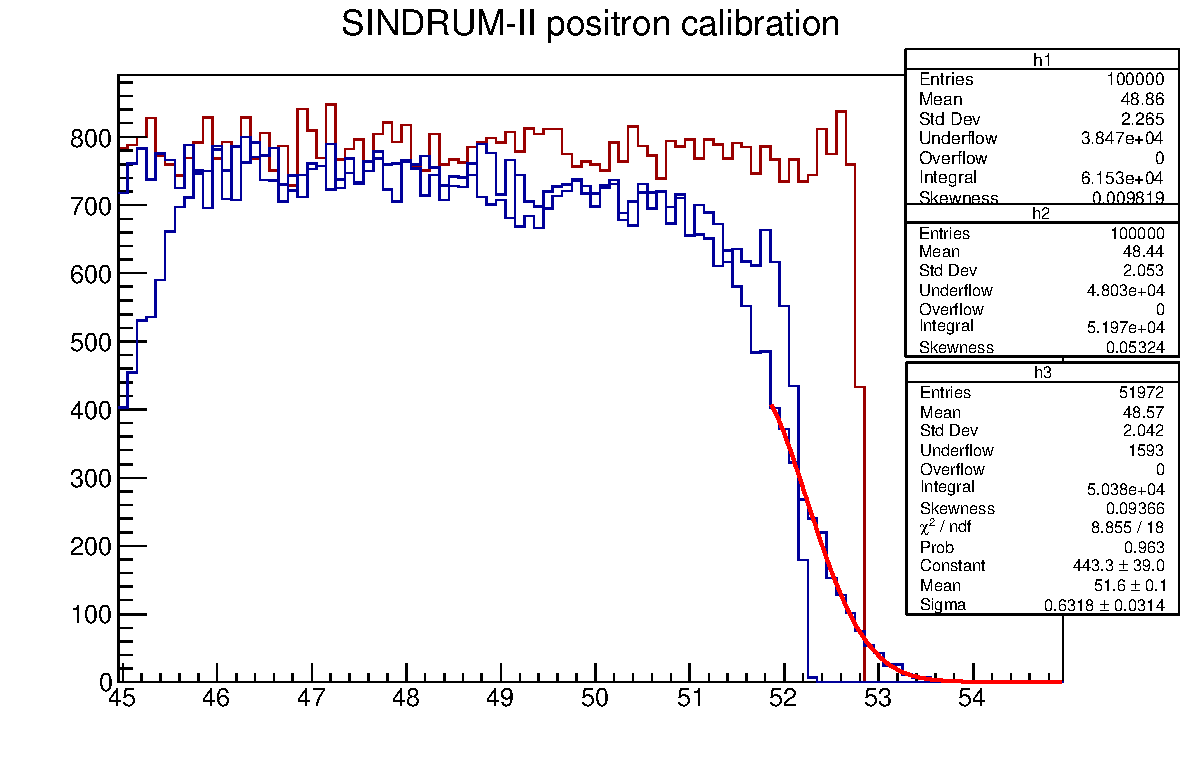
\includegraphics[width=0.99\textwidth]{figures/pdf/sindrum_ii_michel_calibration}
    }
  };
  % \node [text width=6cm, scale=0.8] at (4.5,6.4) {mu2e-18894 by Kevin Lynch and Jim Popp};
\end{tikzpicture}
% \caption{figure} {
\caption{
  \label{fig:sindrum_ii_michel_calibration}
  A flat spectrum with right edge 52.8 MeV is shown in red, the same spectrum convolved with 
  the expected energy losses is in blue, and then this distribution convolved with
  a Gaussian with $\sigma$ = 0.55 MeV is shaded.
}
% \vspace{0.1in}
\end{figure}

%%%%%%%%%%%%%%%%%%%%%%%%%%%%%%%%%%%%%%%%%%%%%%%%%%%%%%%%%%%%%%%%%%%%%%%%%%%%%% 

%%% Local Variables:
%%% mode: latex
%%% TeX-master: t
%%% End:

%%%%%%%%%%%%%%%%%%%%%%%%%%%%%%%%%%%%%%%%%%%%%%%%%%%%%%%%%%%%%%%%%%%%%%%%%%%%%% 
\newpage
\section {Events above 88 MeV and \mumepconv\ signal}


%%%%%%%%%%%%%%%%%%%%%%%%%%%%%%%%%%%%%%%%%%%%%%%%%%%%%%%%%%%%%%%%%%%%%%%%%%%%%% 
\subsection {Positron momentum spectrum}

Figure \ref{fig:ana_step2_ppos_best_fit} overlays the SINDRUM-II positron spectrum on
the \Au{197}\ target with the closure approximation spectrum convolved with the 
parameterized model of the SINDRUM-II detector response.

There are 14 events above 88 MeV/c in the data.

Looking at the data above 94 MeV/c, we can estimate the background due to radiative
pion capture (RPC) and cosmics to be of the order of one event.
The prediction the closure approximation-based RMC model gives is significantly less
than one event above 88 MeV/c.

We therefore need to ask whether the closure approximation reliably
describes the RMC positron spectrum near the endpoint. The closure approximation
doesn't take into account transitions to the exclusive low-lying states of the daughter
nucleus.

In the case of the \Au{197} target, a transition \Au{197} $\ra$ $^{197} \rm Pt$ to
the ground state of the Pt nucleus is allowed. Given that the energy splitting between
an electron and a positron from a photon conversion is almost uniform,
the positron spectrum corresponding to such a transition, in a first approximation,
should be flat. This transistion would have a probability of the order of $10^{-3}$.

\vspace{0.1in}
\begin{tikzpicture}
  \node[anchor=south west,inner sep=0] at (0,0.) {
    % \node[shift={(0 cm,0.cm)},inner sep=0,rotate={90}] at (0,0) {}
    \makebox[\textwidth][c] {
      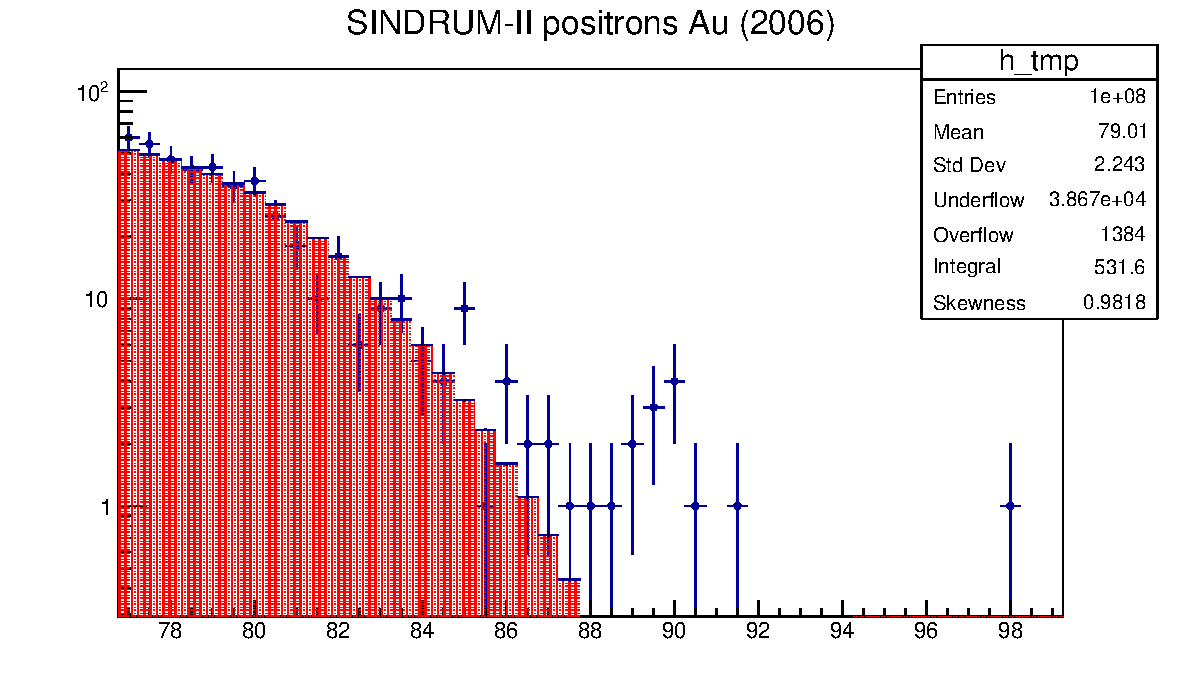
\includegraphics[width=1.0\textwidth]{figures/pdf/ana_step2_ppos_best_fit}
    }
  };
  % \node [text width=6cm, scale=0.8] at (4.5,6.4) {mu2e-18894 by Kevin Lynch and Jim Popp};
\end{tikzpicture}
\captionof{figure} {
  \label{fig:ana_step2_ppos_best_fit}
  Best fit of the SINDRUM-II positron spectrum with the closure approximation
  spectrum convolved with the parameterized model of the SINDRUM-II detector
  response.
}
\vspace{0.1in}

%%%%%%%%%%%%%%%%%%%%%%%%%%%%%%%%%%%%%%%%%%%%%%%%%%%%%%%%%%%%%%%%%%%%%%%%%%%%%%
\subsection{Final states with the broken down daughter nucleus}

As a daughter nucleus produced in the process of radiative muon capture can
breakdown and emit one or several protons or neutrons, one could ask whether
photons from transitions
$$
\mu + \Au{197} \rightarrow \gamma + \nu + ^{197-k}Pt + k \rm ~neutrons
$$
or 
$$
\mu + \Au{197} \rightarrow \gamma + \nu + ^{197-k}A_{Z=78-k} + k \rm ~protons
$$

could have a higher positron energy spectrum endpoint.
Figure ~\ref{fig:pt197_dmass} shows the distributions for mass differences
between the final states consisting of ($^{197-k} \rm Pt$ + k neutrons) and ($^{197-k}A_{Z=78-k}$ + k protons),
and the ground state of $^{197} \rm Pt$. Based on those distributions one can conclude
that events with the most energetic photons and, as such, most energetic 
positrons should correspond to transitions with ``unbroken'' $^{197} \rm Pt$ nucleus
in the final state.

\vspace{0.1in}
\hspace*{-1.3cm}%
\begin{tikzpicture}
  \node[anchor=south west,inner sep=0] at (-2.0,0.0) {
    % \node[shift={(0 cm,0.cm)},inner sep=0,rotate={90}] at (0,0) {}
    % \makebox[\textwidth][c] {
      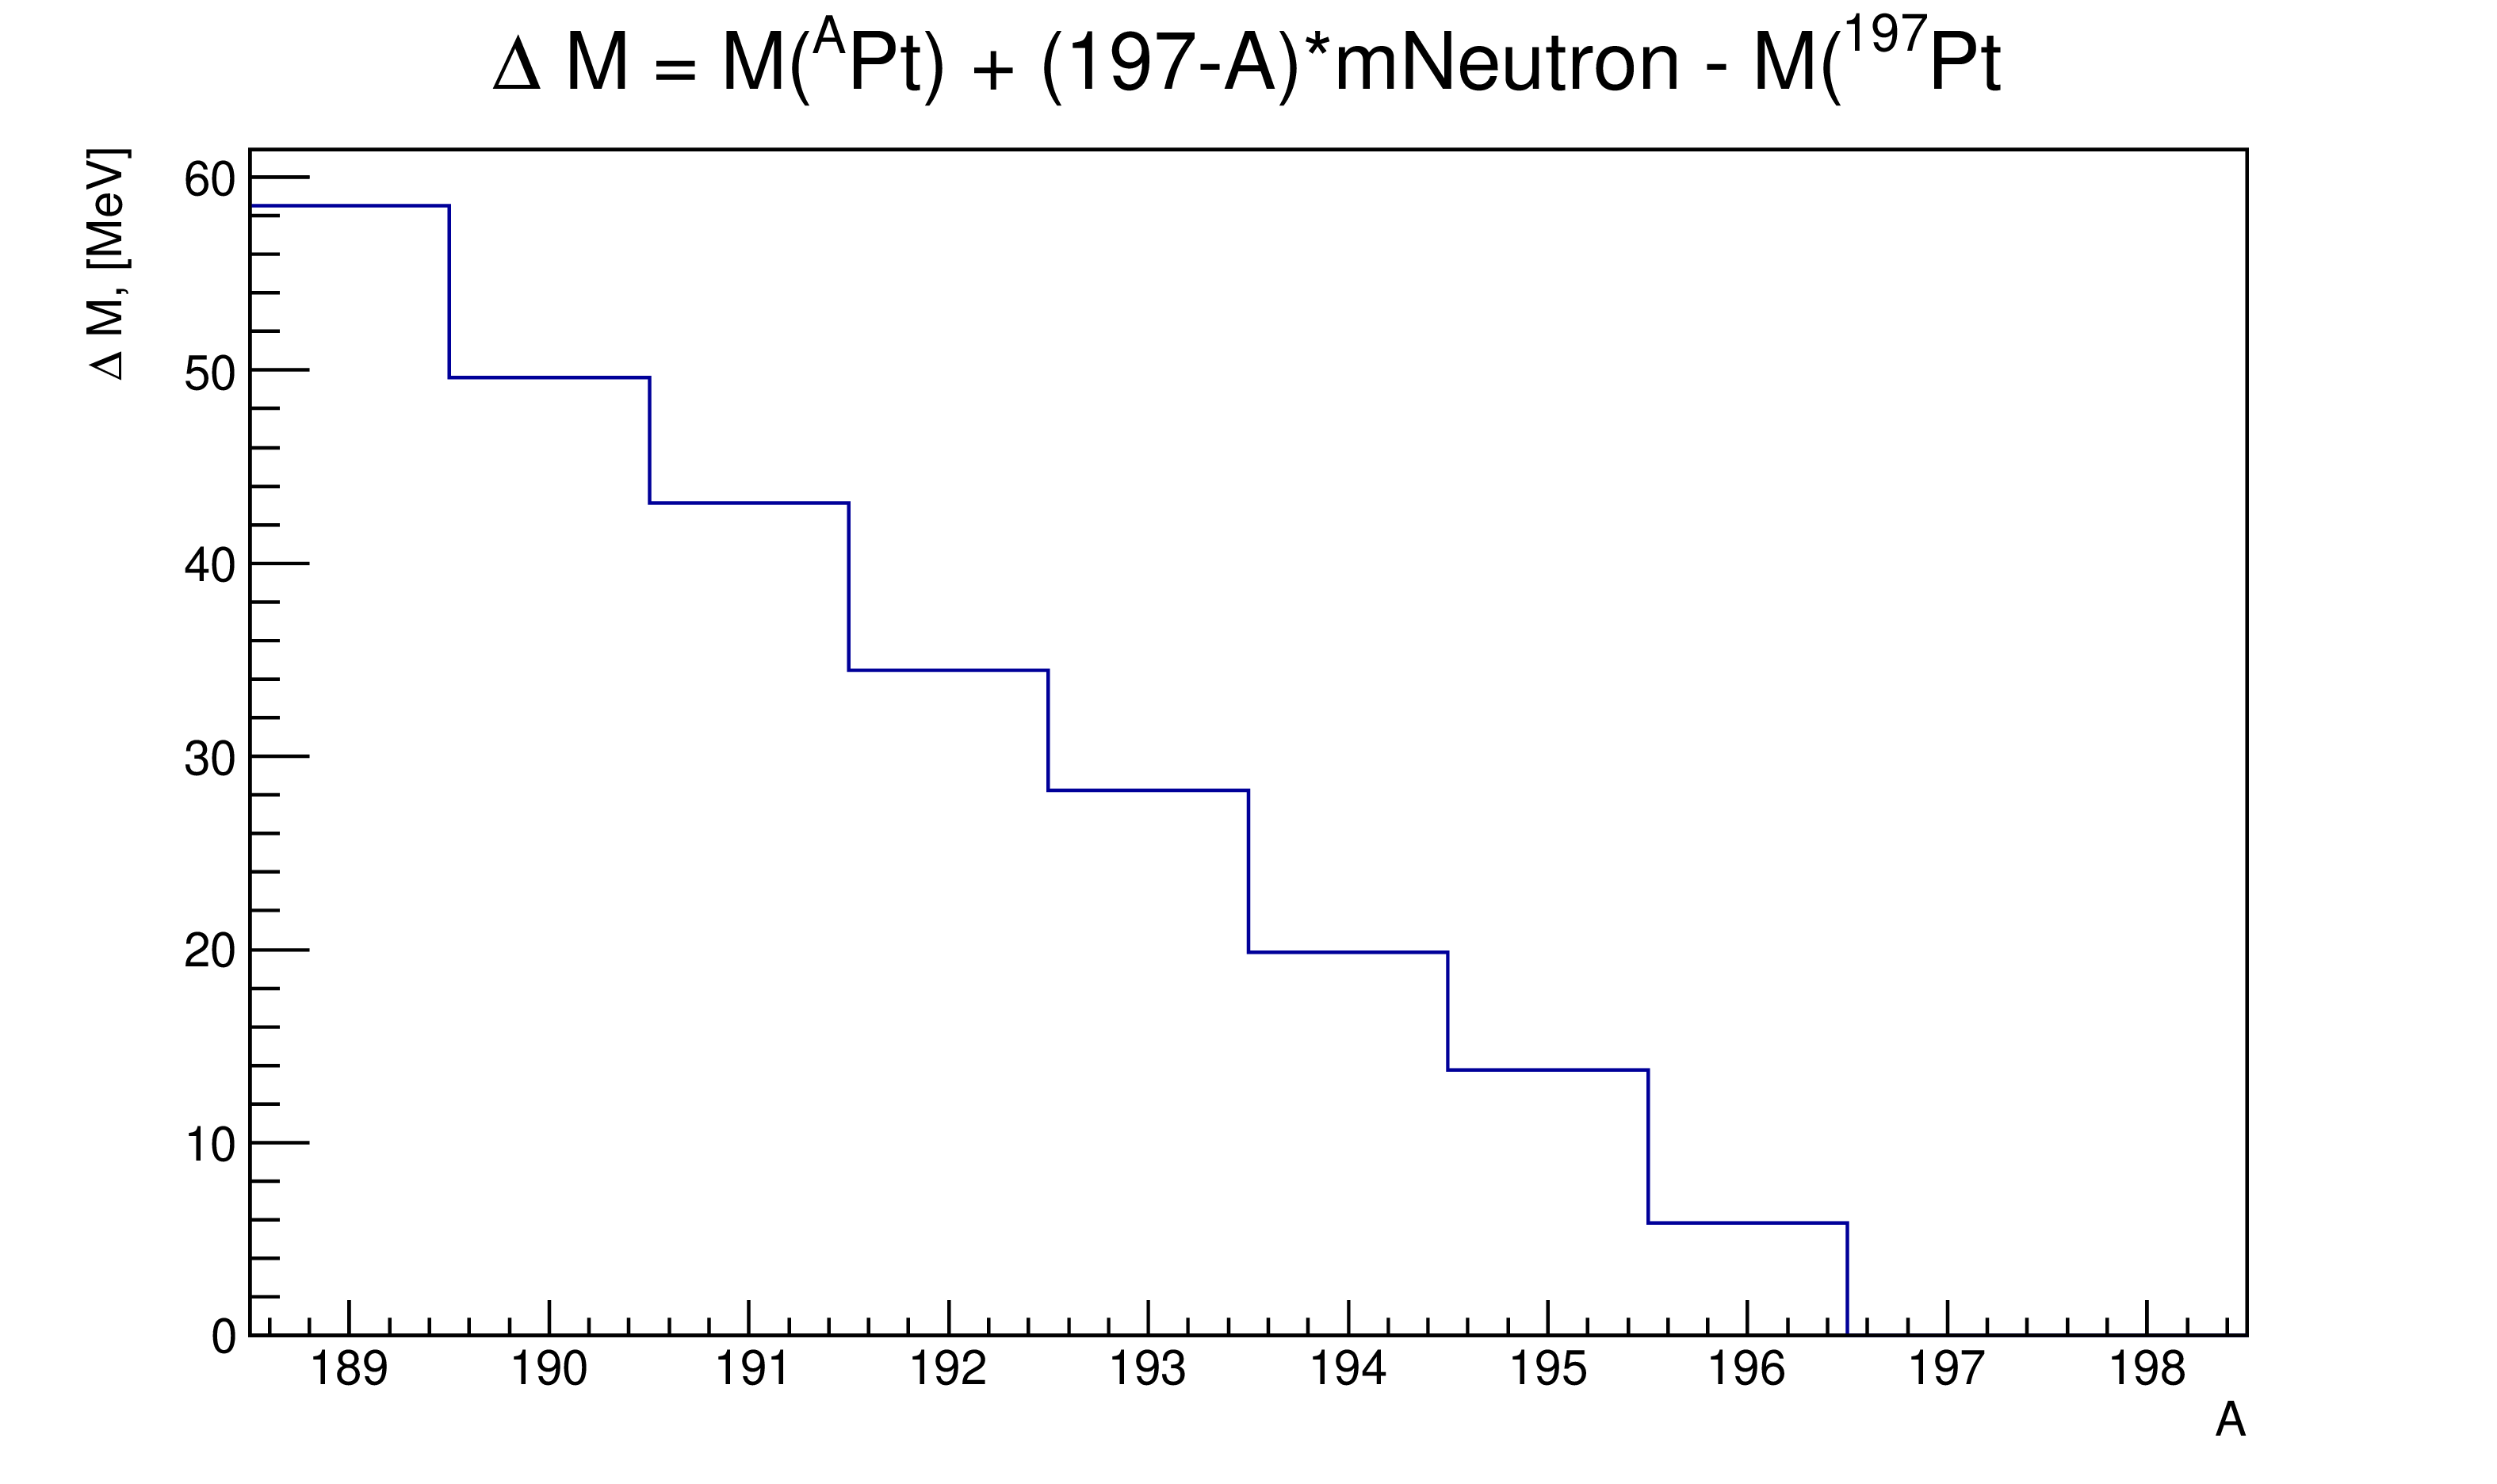
\includegraphics[width=0.6\textwidth]{figures/png/pt197_dmass}
    % }
  };
  \node[anchor=south west,inner sep=0] at (6.0,0.0) {
    % \node[shift={(0 cm,0.cm)},inner sep=0,rotate={90}] at (0,0) {}
    % \makebox[\textwidth][c] {
      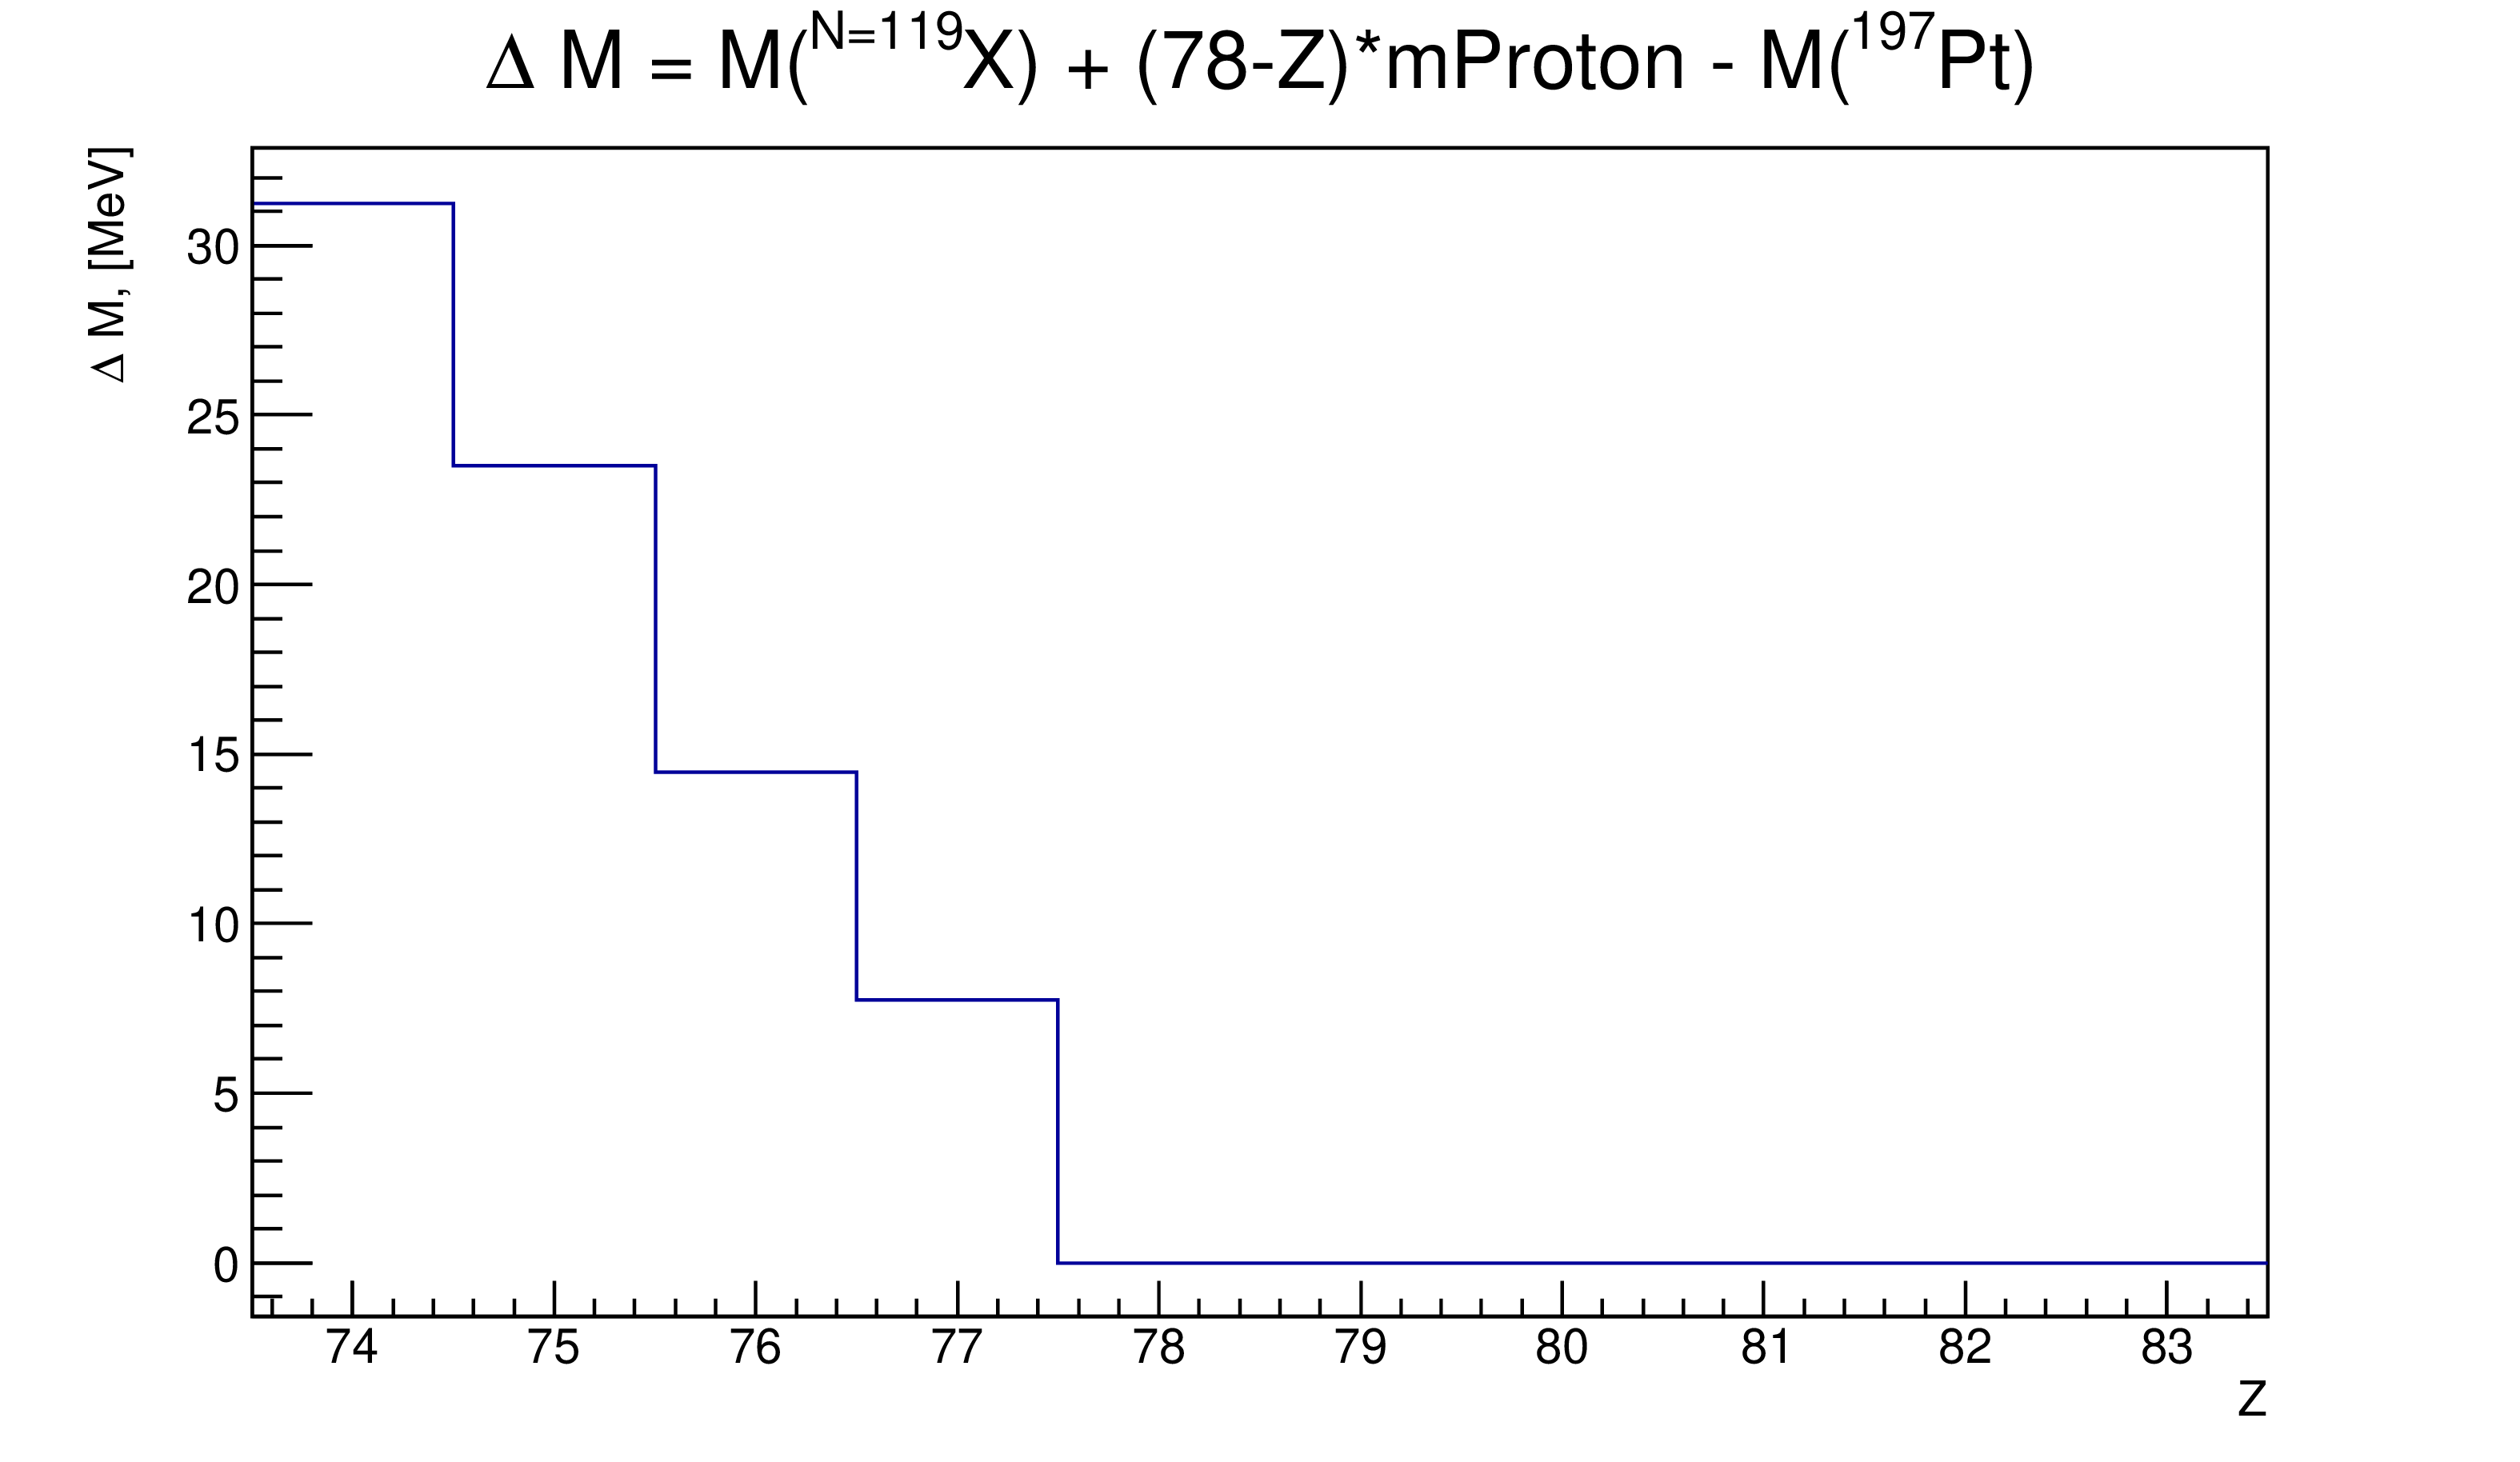
\includegraphics[width=0.6\textwidth]{figures/png/pt197_dmass_n}
    % }
  };
  % \node [text width=6cm, scale=0.8] at (4.5,6.4) {mu2e-18894 by Kevin Lynch and Jim Popp};
\end{tikzpicture}
\captionof{figure} {
  \label{fig:pt197_dmass}
  Mass differences between the final state with the broken down daughter nucleus
  and $^{197} \rm Pt$ for different breakdown scenarios.
  The final state with ``unbroken'' $^{197} \rm Pt$ always has the lowest mass and,
  therefore, the highest photon spectrum endpoint.
}
\vspace{0.1in}

%%%%%%%%%%%%%%%%%%%%%%%%%%%%%%%%%%%%%%%%%%%%%%%%%%%%%%%%%%%%%%%%%%%%%%%%%%%%%%
\subsection {Expected $\mumepconv$ signal in SINDRUM-II detector}

Figure \ref{fig:sindrum_ii_ce_signal} shows expected $\mumemconv[Au]$
conversion signal in the SINDRUM-II detector, digitized from Figure 11 of \cite{sindrum_ii:Bertl2006}. 
The most probable value is at 95.0 MeV/c, consistent with the most probable energy
losses of 0.6 MeV in front of the tracker.

For Au, the expected position of $\mumepconv[Au][Ir]$ is about 3.9 MeV/c lower than
for the $\mumemconv[Au]$ signal; the difference is small enough to not affect the momentum
resolution.
%
We therefore assume that the position and the shape of the $\mu^-\rightarrow e^+$
signal reconstructed in the SINDRUM-II detector can be reproduced by moving
the $\mu^- \rightarrow e^- $signal shown in Figure \ref{fig:sindrum_ii_ce_signal}
by 4 MeV/c towards lower momenta.

\vspace{0.1in}
\begin{tikzpicture}
  \node[anchor=south west,inner sep=0] at (0,0.) {
    % \node[shift={(0 cm,0.cm)},inner sep=0,rotate={90}] at (0,0) {}
    \makebox[\textwidth][c] {
      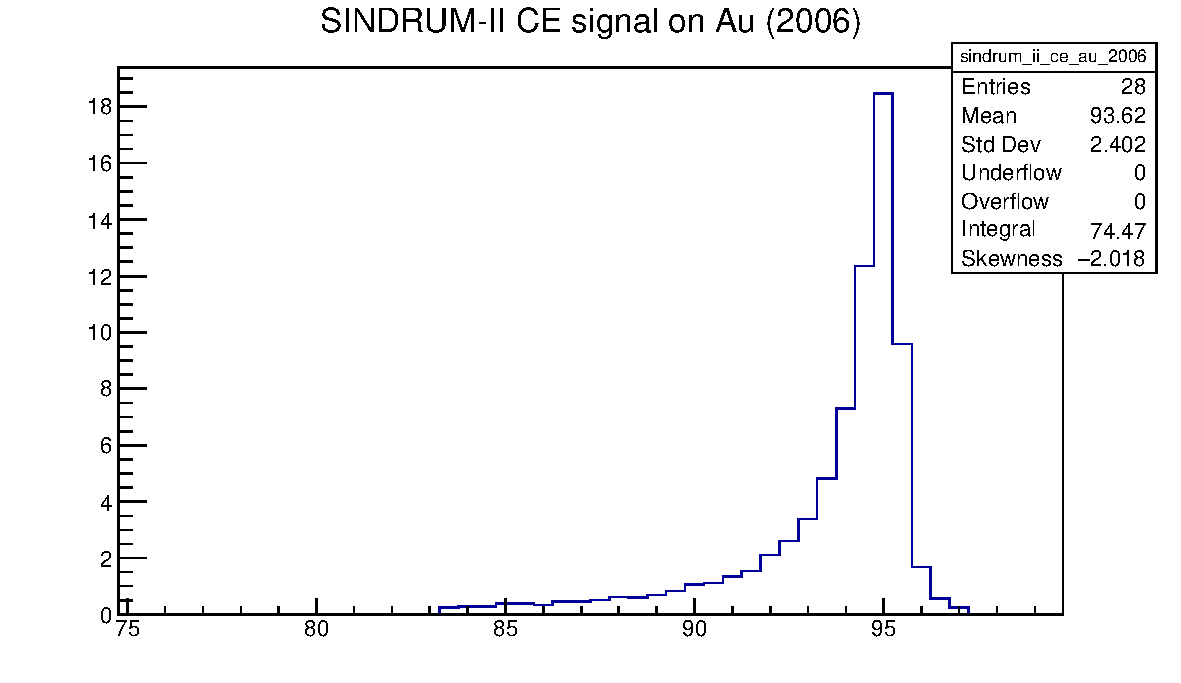
\includegraphics[width=0.99\textwidth]{figures/pdf/sindrum_ii_ce_signal}
    }
  };
  % \node [text width=6cm, scale=0.8] at (4.5,6.4) {mu2e-18894 by Kevin Lynch and Jim Popp};
\end{tikzpicture}
\captionof{figure}{
  \label{fig:sindrum_ii_ce_signal}
  The expected position and shape of the $\mu^- \rightarrow ~e^-$ conversion signal on Au
  in the SINDRUM-II detector.
}
\vspace{0.1in}

Shown in Figure \ref{fig:ana_step2_sindrum_positron_best_fit_signal} is the expected
\mumepconv\ signal on the \Au{197}\ target together with the SINDRUM-II positron spectrum and the
RMC background whose normalization comes from the fit to the data. To guide the eye,
the signal is normalized to 20 events.

Interestingly, the event excess above 88 MeV/c has a shape consistent with the shape
of $\mu^- \rightarrow e^+$ signal; however, the average momentum of the events in the group
is about 1 MeV/c lower than expected from the signal.
The estimated statistical uncertainty on the position of the center of gravity of those
events is 0.24 MeV/c, so the expected position of the $\mu^- \rightarrow e^+$ conversion
signal is about 4$\sigma$ higher than calculated from the data.
This strongly disfavors the exotic ($\mu e$ conversion) interpretation of the excess.

The track charge mis-identification probability in the SINDRUM-II detector
is about 0.2\% \cite{sindrum_ii:Kaulard1998}, and can't explain the positron excess.
%
However, an excess of positron events near the RMC spectrum endpoint could be due
to a process of RMC accompanied by a transition to an exclusive final state
of the $^{197}\rm Pt$ nucleus. As the ground state of \Au{197} has spin parity $3/2^+$
and the ground state of $^{197} \rm Pt$ has spin-parity of $1/2-$, a dipole transition
between these two states is allowed and could result in a mono-energetic photons
with the energy E = 93.8 MeV. A uniform, in the first approximation, distribution
of the electron-positron energy splitting, could result in a a flat contribution 
added, near the endpoint, to the rapidly falling RMC spectrum. 

There are 456 events in the SINDRUM-II positron spectrum with p > 77 MeV/c,
14 out of those have p > 88 MeV/c. Attributing one event - with the highest
momentum - to cosmics, we're left with 13 events with the reconstructed 
positron momenta in the region 88-92 MeV/c. Assuming that all of them are due
to the Au(GS) $\ra$ Pt(GS) RMC transition, and so assuming a flat positron spectrum
from 0 - 93.3 MeV/c, one can estimate the total number
%% Update to reflect positron range
of such events as $13\text{ events}/4\text{ MeV/c}\cdot 92\text{ MeV/c} = 13\cdot 23 \sim\ 300$ events.

For an RMC spectrum with $\kmax = 88$ MeV, shown in Figure ~\ref{fig:rmc_photon_and_positron_spectra}, 
about 14\% of events have photon energies above 57 MeV.
The TRIUMF RMC spectrometer measured 2000-3000 data events per spectrum \cite{}, which translates
into 15,000 - 20,000 events in the whole spectrum per nuclear target. 

Similarly, for $\kmax= 88$ MeV, about $3.3\cdot 10^{-4}$ of all RMC positrons have
p > 77 MeV/c. So assuming momentum-independent efficiency, 442 reconstructed events
would correspond to $1.3\cdot 10^6$ RMC events in the total spectrum and $1.9\cdot 10^5$ RMC events with
the photon p > 57 MeV/c. This is two orders of magnitude higher than
per-target statistics of the TRIUMF RMC spectrometer.

\begin{figure}
  \hspace*{-1.3cm}%
  \begin{tikzpicture}
    \node(base) at (5,0){};
    \node[anchor=south west,inner sep=0] at (0.0,0.) {
      % \node[shift={(0 cm,0.cm)},inner sep=0,rotate={90}] at (0,0) {}
      % \makebox[\textwidth][c] {
      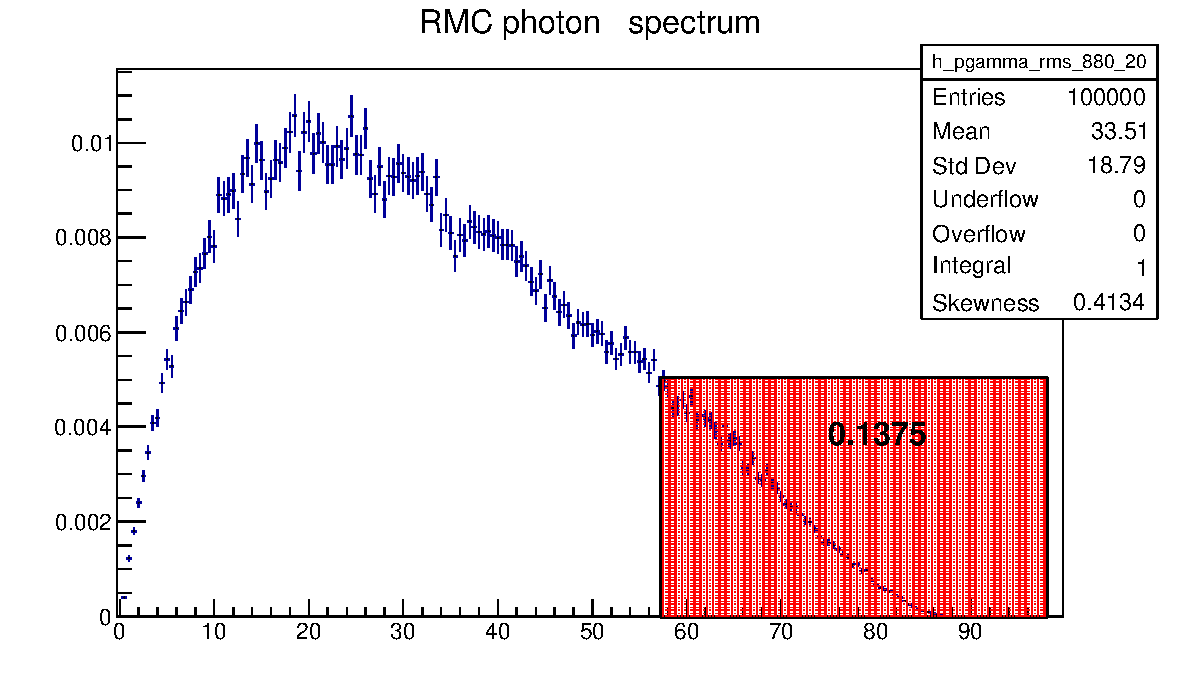
\includegraphics[width=0.6\textwidth]{figures/pdf/rmc_photon_spectrum_kmax_88}
      % }
    };
    \node[anchor=south west,inner sep=0] at (8.1,0.0) {
      % \node[shift={(0 cm,0.cm)},inner sep=0,rotate={90}] at (0,0) {}
      % \makebox[\textwidth][c] {
      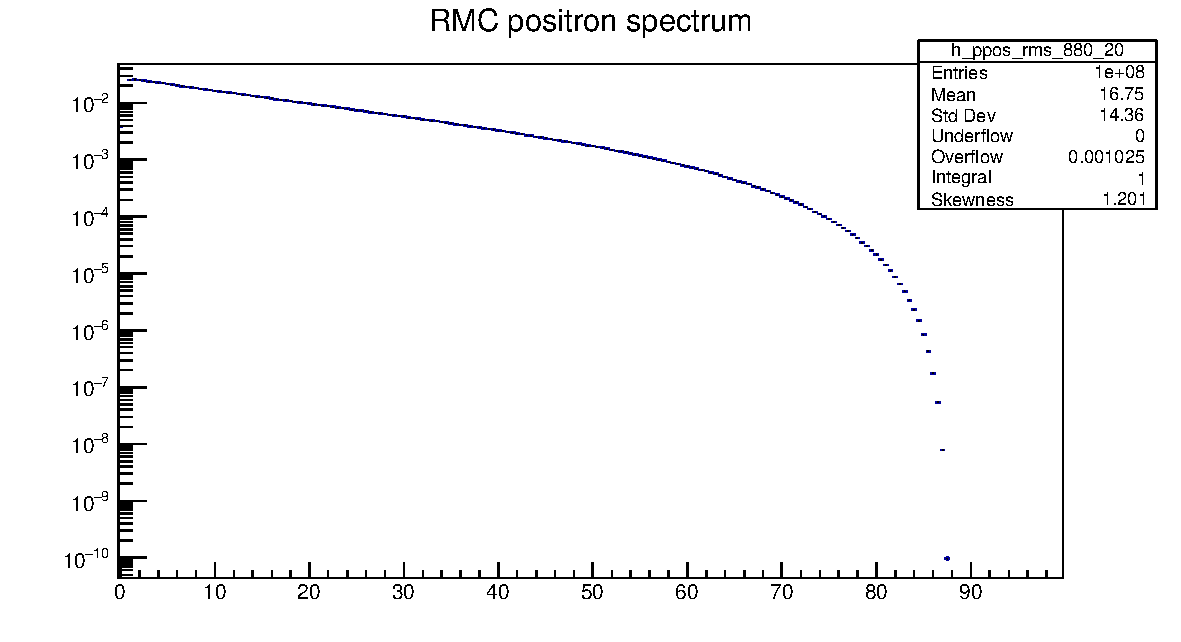
\includegraphics[width=0.6\textwidth]{figures/pdf/rmc_positron_spectrum_kmax_88}
      % }
    };
    % \node [text width=6cm, scale=0.8] at (4.5,6.4) {mu2e-18894 by Kevin Lynch and Jim Popp};
  \end{tikzpicture}
  % \captionof{figure} {
  \caption {
    \label{fig:rmc_photon_and_positron_spectra}
    RMC photon (left) and $e^+$ (right) momentum spectra for $\kmax = 88$ MeV.
  }
\end{figure}


The estimated branching ratio of the exclusive transition would be 
$\sim 3\cdot 10^2/1.3\cdot 10^6 ~ \sim ~ 2\cdot 10^{-4}$, and for the TRIUMF statistics one would expect
$2\cdot 10^4\cdot 2\cdot 10^{-4} ~\sim 5$ events. For a photon energy resolution of FWHM $\sim$ 7 MeV,
it would be rather difficult for the TRIUMF RMC spectrometer group to resolve exclusive
transitions of such strength in the measured spectra. 

\begin{figure}
\begin{tikzpicture}
  \node[anchor=south west,inner sep=0] at (0,0.) {
    % \node[shift={(0 cm,0.cm)},inner sep=0,rotate={90}] at (0,0) {}
    \makebox[\textwidth][c] {
      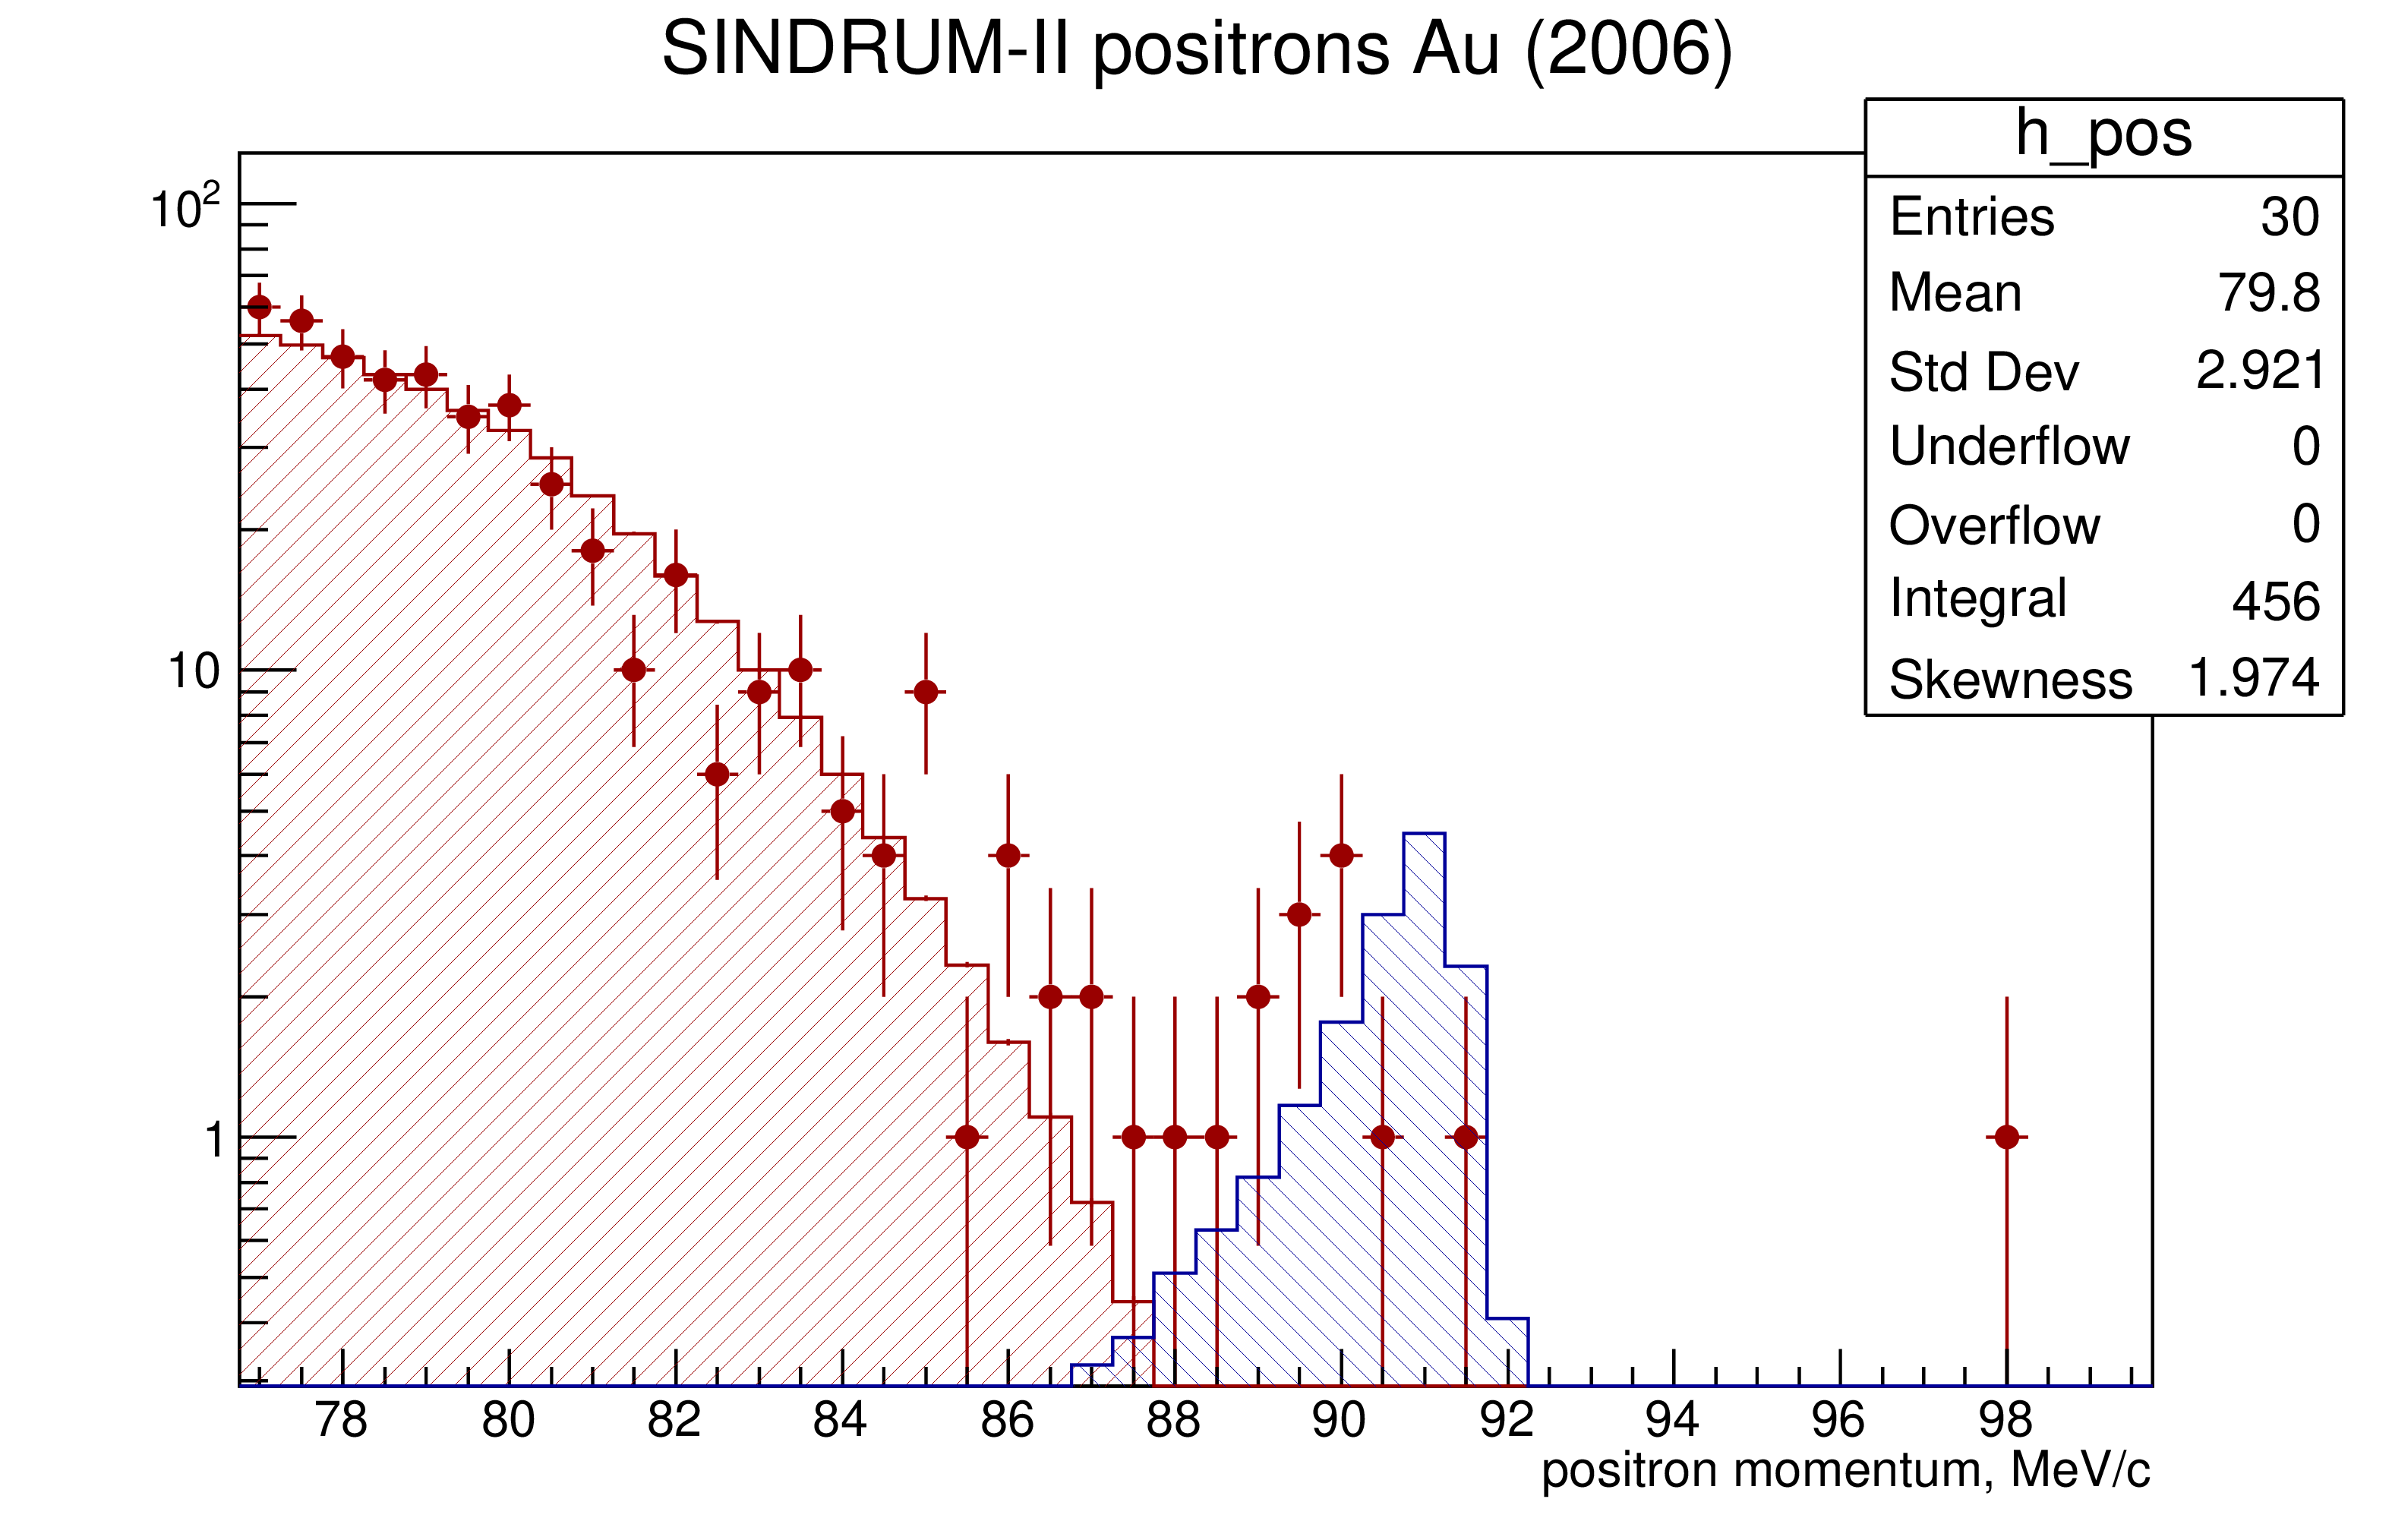
\includegraphics[width=1.0\textwidth]{figures/png/ana_step2_sindrum_positron_best_fit_signal}
    }
  };
  % \node [text width=6cm, scale=0.8] at (4.5,6.4) {mu2e-18894 by Kevin Lynch and Jim Popp};
\end{tikzpicture}
% \captionof{figure} {
\caption {
  \label{fig:ana_step2_sindrum_positron_best_fit_signal}
  SINDRUM-II positron spectrum overlaid with the expected background from RMC
  and a signal from \mumepconv\ normalized to 20 events. Normalization is chosen
  just to guide the eye.
}
\end{figure}


%%%%%%%%%%%%%%%%%%%%%%%%%%%%%%%%%%%%%%%%%%%%%%%%%%%%%%%%%%%%%%%%%%%%%%%%%%%%%%% 
\newpage
\section{ Summary }

\begin{itemize}
\item
  assuming that the RMC spectrum is described by the closure approximation,
  SINDRUM-II positron spectrum on Au target shows a statistically significant
  excess of events (roughly, 13 events with 1 expected) over the background
\item
  The limit on BGR comes from cosmics and RPC, RMC $\ll$ 1  event.
\item
  The excess looks like a bump with the width consistent with the detector
  resolution.
\item
  The expected position of $\mu^- \rightarrow e^+$ conversion signal on Au is
  about 1 MeV/c or, statistically, 4*$\sigma_P$ higher, which strongly discourages
  the exotic interpretation.
\item
  The excess could be due to an exclusive RMC transition Au(GS) $\ra$ Pt (GS)
  with the branching fraction of about $2\cdot10^{-4}$, which is spin/parity
  allowed. Given the statistics and the resolution of the published RMC
  measurements, such a transition would not be resolved. 
\item
  This observation has significant implications for the upcoming
  searches
  for the process of $\mu^- \rightarrow e^+$ conversion. 
  To fully exploit the physics potential of experiments like Mu2e and COMET,
  a better theoretical understanding of the endpoint of the RMC spectrum
  on nuclei is needed. 
\item
  Without that, the sensitivity for these searches might be limited by the presently unknown
  dipole RMC transitions to exclusive states of the daughter nuclei. 
\end{itemize}

%%%%%%%%%%%%%%%%%%%%%%%%%%%%%%%%%%%%%%%%%%%%%%%%%%%%%%%%%%%%%%%%%%%%%%%%%%%%%%% 
% \section{ Acknowledgements }
% 
% We want to thank ...
% 
%%%%%%%%%%%%%%%%%%%%%%%%%%%%%%%%%%%%%%%%%%%%%%%%%%%%%%%%%%%%%%%%%%%%%%%%%%%%%%

\appendix
\section{$\mumepconv[Au][Ir]$ energy calculation}
We consider only the ground state conversion process. 
For this, the conversion energy is given by:
$$
E_{e^+} = m_\mu - B_\mu - E_{recoil} - \Delta_{Z-2}
$$

where $m_\mu$ is the muon mass, $B_\mu$ is the binding energy of the 1s energy level,
$E_{recoil}$ is the energy of the recoiling nucleus, and $\Delta_{Z-2}$ is the difference
between the incoming and outgoing nuclear masses. 

\begin{table}[h]
  \begin{center}
    \begin{tabular}{|l || c |}
      \hline
      Parameter & Value  \\
      \hhline{|=||=|}
      $m_\mu$ & 105.6583745(24) MeV/c$^2$\\
      \hline
      $m_e$   & 0.5109989461(31) MeV/c$^2$\\ %6.1e-9
      \hline
      $1u$ & 931.49410242(28) MeV/c$^2$ \\ %3e-10
      \hline
      $B_\mu$ & 10081.23 keV\\ %?
      \hline
      $A_r(\Au{197})$ & 196.96656879(71) u \\%~1e-8
      \hline
      $M_N(\Au{197})$ & 183432.828(1) MeV/c$^2$\\%~1-2 e-8
      \hline
      $A_r(\Ir{197})$ & 196.969 655(22) u \\%~1e-7
      \hline
      $M_N(\Ir{197})$ & 183436.725(21) MeV/c$^2$ \\%~1e-7
      \hline
      $\Delta_{Z-2}$ & 3.897(21) MeV/c$^2$ \\
      \hline
    \end{tabular}
  \end{center}
  \caption{Parameters used in the $\mumepconv[Au][Ir]$ positron energy calculation.}
  \label{table:parameters}
\end{table}

Since the muon orbit is $\sim$ 200 times closer to the nucleus than the electrons',
one can assume the electrons do not contribute to the muon capture process. Therefore,
the electron masses are not considered and instead only the nuclear masses are used:
$M_N = M_A-Z\cdot m_e$, where $M_A=A_r\cdot u$, $A_r$ is the relative mass, 
u is the atomic mass unit, and $m_e$ is the electron mass.

The recoiling energy is given by considering the two body decay: $N(\mu^-+\Au{197}) \ra e^+ + \Ir{197}$.
Considering the rest frame of the muonic gold atom, the decay products must satisfy
$p_{e^+} + p_{^{197}Ir} = p_{o} = 0$. The energy of the iridium mucleus is then given by:
$$
E_{^{197}Ir} = \frac{M^2 + M_N(\Ir{197})^2 - m_e^2}{2M} = E_{recoil} + M_N(\Ir{197})
$$
where M is the mass of the muonic gold nucleus system, $M_N(\Au{197}) + m_\mu - B_\mu = 183528.405$ MeV/c$^2$.
Using the parameters in Table \ref{table:parameters}, we get $E_{recoil} = 0.023$ MeV.

Combining these together, the $\mumepconv[Au][Ir]$ positron energy for the ground state
transition is $E_{e^+} = 91.657(21)$ MeV, where the uncertainty on $B_\mu$ is assumed to be $\sim$0.001 MeV.

\bibliographystyle{unsrtnat}
\bibliography{clfv,dio,radiative_muon_capture}
%% \printbibliography
\end{document}


% ------------------------------------------------------------------------------
% templates
% ------------------------------------------------------------------------------
% Table ~\ref{table:summary} gives summary the numbers used in this study.
% 
% \hspace{-0.1in}
% \begin{table}[htbp]
%   \label{table:summary}
%   \begin{center} 
%     {\renewcommand{\arraystretch}{1.0}   % change 1.0 to 1.1 to increase the spacing between the table lines
%       \begin{tabular}{|c|c|c|c|}
%         \hline
%                             & default TS geometry & misaligned TS geometry   &  Ratio(default/misaligned)    \\ 
%         \hline
%         $N_{POT}$            &  $4.96 \cdot 10^6$  &    $5.00 \cdot 10^6$      &   0.992   \\ 
%         $N_{\mu}^{TS3u}$      &  65648              &     61354                 &   1.070   \\ 
%         $N_{\mu}^{TS5}$       &  28517              &     27351                 &   1.043   \\ 
%         $N_{\mu}^{ST}$        &  8868               &      8396                 &   1.056   \\ 
%         $N_{\mu}^{ST}/N_{POT}$ &  $1.79 \pm 0.02$    &    $1.68 \pm 0.02$        &   $1.065 \pm 0.03$        \\ 
%         \hline
%       \end{tabular}
%     }
%   \end{center}
%   \caption{
%     Muons rates at different points of the Mu2e beamline and stopping muon rates for nominal and 
%     misaligned TS geometries
%   }
%   % \vspace{0.5in}
% \end{table}
